\documentclass[%
	pdftex,
	oneside,		% Einseitiger Druck.
	12pt,			% Schriftgroesse
	parskip=half,	% Halbe Zeile Abstand zwischen Absätzen.
	headsepline,	% Linie nach Kopfzeile.
	%footsepline,	% Linie vor Fusszeile.
	abstracton,	    % Abstract Überschriften
	ngerman,		% Translator
]{scrartcl}

% Zeichencodierung
\usepackage[utf8]{inputenc}
\usepackage[T1]{fontenc}
 
\newcommand{\pdftitel}{Konzeption und Entwicklung einer digitalen Funk-, LED-Uhr}
\newcommand{\autor}{Tobias Schöneberger, Matthis Hauschild}
\newcommand{\arbeit}{Studienarbeit}
%falls pdftitel = titel der Arbeit
\newcommand{\titel}{\pdftitel}
%bei unterschiedlichen Titeln
%\newcommand{\titel}{In der Regel haben wir einen zweizeiligen
% Bachelorthesistitel}
\newcommand{\kurs}{TIT10AID}
\newcommand{\datumAbgabe}{Juni 2013}
\newcommand{\abgabeort}{Stuttgart}
\newcommand{\studiengang}{Angewandte Informatik}
\newcommand{\dhbw}{Stuttgart}
\newcommand{\betreuer}{Prof. Dr. Karl Friedrich Gebhardt}
\newcommand{\gutachter}{Prof. Dr. Karl Friedrich Gebhardt}
\newcommand{\zeitraum}{12 Wochen}
\newcommand{\arbeitsart}{\arbeit}


%Seitengroesse
\usepackage{fullpage} 

%Zeilenumbruch und mehr
\usepackage[activate]{microtype}


% Zeilenabstand
\usepackage[onehalfspacing]{setspace}

% Index-Erstellung
%\usepackage{makeidx}

% Lokalisierung (neue deutsche Rechtschreibung)
\usepackage[ngerman]{babel}  
 
% Anführungszeichen 
\usepackage[babel,german=quotes]{csquotes}
%\usepackage[style=swiss]{csquotes}


% Spezielle Tabellenform fuer Deckblatt
\usepackage{longtable}
\setlength{\tabcolsep}{10pt} %Abstand zwischen Spalten
\renewcommand{\arraystretch}{1.5} %Zeilenabstand

% Grafiken
\usepackage{graphicx}

%Farben
\usepackage{color}
\definecolor{sh_comment}{rgb}{0.12, 0.38, 0.18 } %adjusted, in Eclipse: {0.25, 0.42, 0.30 } = #3F6A4D
\definecolor{sh_keyword}{rgb}{0.37, 0.08, 0.25}  % #5F1441
\definecolor{sh_string}{rgb}{0.06, 0.10, 0.98} % #101AF9

%\usepackage{fancyhdr}

\usepackage{bibgerm}
\usepackage{longtable}
% für textumflossene Grafiken
\usepackage{wrapfig} 

% Fussnoten
\usepackage[perpage, hang, multiple, stable]{footmisc}

% Verschiedene Schriftarten
%\usepackage{goudysans}
\usepackage{lmodern}
%\usepackage{libertine}
%\usepackage{palatino} 

% Hurenkinder und Schusterjungen verhindern
% http://projekte.dante.de/DanteFAQ/Silbentrennung
\clubpenalty=10000
\widowpenalty=10000
\displaywidowpenalty=10000

\newcommand{\degree}{\ensuremath{^\circ}}

% Titel, Autor und Datum
\title{\titel}
\author{\autor}
\date{\datum}

% PDF Einstellungen
\usepackage[%
	pdftitle={\pdftitel},
	pdfauthor={\autor},
	pdfsubject={\arbeit},
	pdfcreator={pdflatex, LaTeX with KOMA-Script},
	pdfpagemode=UseOutlines, % Beim Oeffnen Inhaltsverzeichnis anzeigen
	pdfdisplaydoctitle=true, % Dokumenttitel statt Dateiname anzeigen.
	pdflang=de % Sprache des Dokuments.
]{hyperref} 

 \usepackage{listings}
 \usepackage{courier}
 \lstset{
         basicstyle=\small\ttfamily, % Standardschrift
         numbers=left,               % Ort der Zeilennummern
         numberstyle=\tiny,          % Stil der Zeilennummern
         %stepnumber=2,               % Abstand zwischen den Zeilennummern
         numbersep=5pt,              % Abstand der Nummern zum Text
         tabsize=2,                  % Groesse von Tabs
         lineskip=-2pt,
         extendedchars=true,         %
         breaklines=true,            % Zeilen werden Umgebrochen
         keywordstyle=\color{sh_keyword}\bfseries,
            frame=b,         
 %        keywordstyle=[1]\textbf,    % Stil der Keywords
 %        keywordstyle=[2]\textbf,    %
 %        keywordstyle=[3]\textbf,    %
 %        keywordstyle=[4]\textbf,   \sqrt{\sqrt{}} %
         stringstyle=\color{sh_string}\ttfamily, % Farbe der String
         commentstyle=\color{sh_comment},
         showspaces=false,           % Leerzeichen anzeigen ?
         showtabs=false,             % Tabs anzeigen ?
         xleftmargin=17pt,
         framexleftmargin=17pt,
         framexrightmargin=5pt,
         framexbottommargin=4pt,
         %backgroundcolor=\color{lightgray},
         showstringspaces=false      % Leerzeichen in Strings anzeigen ?        
 }
 \lstloadlanguages{% Check Dokumentation for further languages ...
         %[Visual]Basic
         %Pascal
         C
         %C++
         %XML
         %HTML
         %Java
 }
\usepackage{caption}
\DeclareCaptionFont{white}{\color{white}}
\DeclareCaptionFormat{listing}{\colorbox[cmyk]{0.43, 0.35, 0.35,0.01}{\parbox{\textwidth}{\hspace{15pt}#1#2#3}}}
\captionsetup[lstlisting]{format=listing,labelfont=white,textfont=white, singlelinecheck=false, margin=0pt, font={bf,footnotesize}}

\renewcommand{\figurename}{Abb.}

\begin{document}
\renewcommand{\figurename}{Abb.}
	% Deckblatt
	\begin{spacing}{1}
		\begin{titlepage}
	\begin{longtable}{p{.4\textwidth} p{.4\textwidth}}
	  {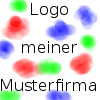
\includegraphics[height=2.6cm]{images/logo.png}} & 
	  {
\includegraphics[height=2.6cm]{images/dhbw.png}}
	\end{longtable}
	\enlargethispage{20mm}
	\begin{center}
	  \vspace*{12mm}	{\LARGE\bf \titel }\\
	  \vspace*{12mm}	{\large\bf \arbeit}\\
	  \vspace*{12mm}	für die Prüfung zum\\
	  \vspace*{3mm} 	{\bf \abschluss}\\
	  \vspace*{12mm}	des \studiengang\\
	  \vspace*{3mm} 	an der Dualen Hochschule Baden-Württemberg \dhbw\\
	  \vspace*{12mm}	von\\
	  \vspace*{3mm} 	{\large\bf \autor}\\
	  \vspace*{12mm}	\datumAbgabe\\
	\end{center}
	\vfill
	\begin{spacing}{1.2}
	\begin{tabbing}
		mmmmmmmmmmmmmmmmmmmmmmmmmm     \= \kill
		\textbf{Bearbeitungszeitraum}  \>  \zeitraum\\
		\textbf{Matrikelnummer, Kurs}  \>  \martrikelnr, \kurs\\
		\textbf{Ausbildungsfirma}      \>  \firma, \firmenort\\
		\textbf{Betreuer}              \>  \betreuer\\
		\textbf{Gutachter}             \>  \gutachter
	\end{tabbing}
	\end{spacing}
\end{titlepage}

	\end{spacing}
	\newpage

	% Sperrvermerk
	\renewcommand{\thepage}{\Roman{page}} 
	\setcounter{page}{1}

	% Erklärung
	\thispagestyle{empty}

\section*{Erklärung}
% http://www.se.dhbw-mannheim.de/fileadmin/ms/wi/dl_swm/dhbw-ma-wi-organisation-bewertung-bachelorarbeit-v2-00.pdf
\vspace*{2em}

Wir erklären hiermit ehrenwörtlich: \\
\begin{enumerate}
\item dass wir unsere {\arbeitsart} mit dem Thema
{\itshape \titel } ohne fremde Hilfe angefertigt haben;
\item dass wir die Übernahme wörtlicher Zitate aus der Literatur sowie die
Verwendung der Gedanken anderer Autoren an den entsprechenden Stellen innerhalb
der Arbeit gekennzeichnet haben;
\item dass wir unsere {\arbeitsart} bei keiner anderen Prüfung vorgelegt habe;
\item dass die eingereichte elektronische Fassung exakt mit der eingereichten schriftlichen Fassung
übereinstimmt.
\end{enumerate}

Wir sind uns bewusst, dass eine falsche Erklärung rechtliche Folgen haben wird.

\vspace{3em}

\abgabeort, \datumAbgabe
\vspace{6em}

\begin{tabular}[h]{p{5cm} p{2cm} p{5cm}}
  \hline
	Matthis Hauschild & &Tobias Schöneberger \\
\end{tabular} 

	\newpage
	
	\tableofcontents
	\newpage 
	
	\renewcommand{\thepage}{\arabic{page}}
	\setcounter{page}{1}
	 
	\section{Einleitung}
\subsection{Motivation}
TODO

\subsection{Umfang}
TODO 
	\section{Anforderungen}
TODO
	\section{Technische Grundlagen}
\subsection{DCF77}\label{sec_dcfgrund}
DCF77 ist ein Zeitzeichensender in Mainhausen bei Frankfurt, der seit dem ersten Januar 1959 die Uhrzeit auf der Langwellenfrequenz von 77,5 kHz sendet. Bei Sendeanlagen, die über Ländergrenzen hinaus senden, muss das Rufzeichen in der internationalen Frequenzliste eingetragen sein und das Kennzeichen des jeweiligen Landes enthalten. Deshalb wurde DCF77 gewählt, wobei das D für Deutschland steht. Der Buchstabe C war früher ein Kennzeichen für Langwelle und das F steht für Frankfurt. Da die Sendeanlage in Mainhausen mehrere Sender hat, wurde noch die Zahl 77 als Andeutung auf die Trägerfrequenz (77,5 kHz) gewählt\footnote{vgl. \cite{dcf77}, Seite 349f.}.

Das Zeitsignal wird jede Minute wiederholt und kodiert Zeit- sowie Datumsinformationen. Dabei wird jede Sekunde ein Bit übertragen. Dies geschieht durch Amplitudenmodulation. Jede Sekunde wird die Amplitude der Trägerwelle für 100 ms (logisch 0) oder 200 ms (logisch 1) auf etwa 25 \% abgesenkt. Lediglich in Sekunde 59 wird die Amplitude zur Erkennung der neuen Minute nicht abgesenkt. Tabelle \ref{tbl_dcf77kod} zeigt die Bedeutung der gesendeten Bits im DCF77-Signal\footnote{vgl. \cite{dcf77}, Seite 351ff.}.
\newpage
%
\renewcommand{\arraystretch}{1}
\begin{longtable}{|l|l|}
\hline Bit & Bedeutung\\\hline\hline\endhead
\hline\endfoot\endlastfoot
%
0 & Minutenanfang\\\hline
1 - 14 & verschlüsselte Wetterinformationen\\\hline
15 & Rufbit: Ankündigung, wenn von Reserveantenne gesendet wird\\\hline
16 & A1: Wechsel von/zur Sommerzeit bei nächstem Stundenwechsel\\\hline
17 - 18 & Zeitzonenbits: 01: MEZ, 10: MESZ\\\hline
19 & A2: Schaltsekunde bei nächstem Stundenwechsel\\\hline
20 & S: Startbit (immer logisch 1)\\\hline
21 & Minutenbit, Wertigkeit 1\\\hline
22 & Minutenbit, Wertigkeit 2\\\hline
23 & Minutenbit, Wertigkeit 4\\\hline
24 & Minutenbit, Wertigkeit 8\\\hline
25 & Minutenbit, Wertigkeit 10\\\hline
26 & Minutenbit, Wertigkeit 20\\\hline
27 & Minutenbit, Wertigkeit 40\\\hline
28 & Prüfbit für Minuten, Even Parity\\\hline
29 & Stundenbit, Wertigkeit 1\\\hline
30 & Stundenbit, Wertigkeit 2\\\hline
31 & Stundenbit, Wertigkeit 4\\\hline
32 & Stundenbit, Wertigkeit 8\\\hline
33 & Stundenbit, Wertigkeit 10\\\hline
34 & Stundenbit, Wertigkeit 20\\\hline
35 & Prüfbit für Stunden, Even Parity\\\hline
36 & Kalendertag, Wertigkeit 1\\\hline
37 & Kalendertag, Wertigkeit 2\\\hline
38 & Kalendertag, Wertigkeit 4\\\hline
39 & Kalendertag, Wertigkeit 8\\\hline
40 & Kalendertag, Wertigkeit 10\\\hline
41 & Kalendertag, Wertigkeit 20\\\hline
42 & Wochentag, Wertigkeit 1\\\hline
43 & Wochentag, Wertigkeit 2\\\hline
44 & Wochentag, Wertigkeit 4\\\hline
45 & Kalendermonat, Wertigkeit 1\\\hline
46 & Kalendermonat, Wertigkeit 2\\\hline
47 & Kalendermonat, Wertigkeit 4\\\hline
48 & Kalendermonat, Wertigkeit 8\\\hline
49 & Kalendermonat, Wertigkeit 10\\\hline
50 & Kalenderjahr, Wertigkeit 1\\\hline
51 & Kalenderjahr, Wertigkeit 2\\\hline
52 & Kalenderjahr, Wertigkeit 4\\\hline
53 & Kalenderjahr, Wertigkeit 8\\\hline
54 & Kalenderjahr, Wertigkeit 10\\\hline
55 & Kalenderjahr, Wertigkeit 20\\\hline
56 & Kalenderjahr, Wertigkeit 40\\\hline
57 & Kalenderjahr, Wertigkeit 80\\\hline
58 & Prüfbit für Kalenderjahr, Even Parity\\\hline
59 & Markierung der neuen Minute, keine Amplitudenabsenkung\\\hline
\caption{Erläuterung der Bits im DCF77-Zeitsignal\footnotemark}\label{tbl_dcf77kod}
\end{longtable}
\footnotetext{vgl. \cite{dcf77}, Seite 352f.}
%
\subsection{LED Matrix}
Unter LED Matrix versteht man die Ansteurung von LEDs in Zeilen und Spalten. Dabei werden alle Anoden zu Spalten und alle Kathoden zu Zeilen
verbunden.\footnote{Es kann natürlich auch die Kathode für Spalten und die
Anode für Zeilen verwendet werden.} Im Vergleich zu einer Einzelansteuerung
bietet die LED Matrix den großen Vorteil, dass bei einer Matrix mit $N$ Spalten
und $M$ Zeilen nur $N+M$ statt $N*M$ Leitungen verwendet werden.

\begin{wrapfigure}{r}{0.45\textwidth}
  \vspace{-25pt}
  \begin{center}
    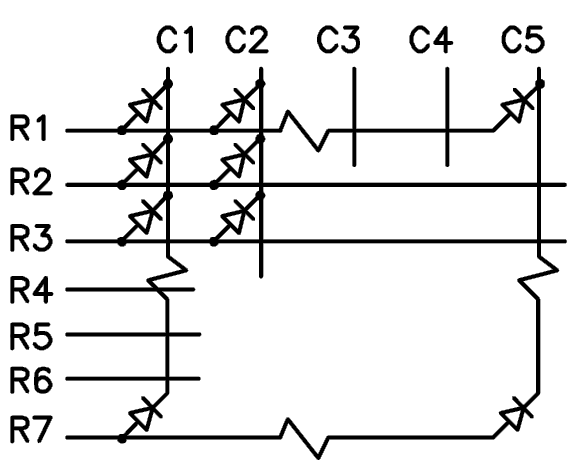
\includegraphics[width=0.42\textwidth]{skizzen/led_matrix_5x7.png}
  \end{center}
  \vspace{-20pt}
  \captionof{figure}{5x7 LED Matrix}
\end{wrapfigure}

Die LED Matrix
wird dann zeilenweise oder spaltenweise im Multiplexbetrieb angesteuert. Das bedeutet, dass nacheinander eine der Spalten mit GND versorgt wird und die anderen Spalten unbeschalten sind (keine Verbindung zu GND). Nun können in dieser Spalte durch Anlegen von Spannung an den entsprechenden Zeilen LEDs angeschaltet werden. 
Dieser Vorgang wird für alle Spalten durchgeführt, das bedeutet es leuchten zu
einem bestimmten Zeitpunkt immer nur die LEDs einer Spalte. Durch das schnelle
Umschalten zwischen den Spalten und die Trägheit des menschlichen Auges entsteht
die Illusion, dass auf der kompletten LED Matrix die LEDs aktiviert sind.
Als Nachteil aus dieser Beschaltung ergibt sich die verringerte Helligkeit, da
die LEDs bei $N$ Spalten nur noch $\frac{1}{N}$ der Zeit leuchten.

Der Helligkeitsverlust kann durch höheren Stromfluss zum Teil kompensiert
werden. Das bedeutet bei $N$ Spalten werden die LEDs mit einem Pulsstrom von
$N*Nennstrom$ betrieben. Durch die Dunkelphasen kann das aktive Substrat
zwischen den Pulsen ausreichend abkühlen. Generell kann dies bis zum ca.
zehnfachen Nennstrom (200 mA bei einer gewöhnlichen 20 mA LED) durchgeführt
werden.\footnote{vgl. \cite{ledMatrix}}

\subsection{Pulsweitenmodulation}\label{sec_pulsweitenmodulation}
Pulsweitenmodulation bezeichnet eine Modulationstechnik in der die Weite des
Pulses bei einer gleichbleibenden Periode verändert wird (siehe \ref{pwm_schma}).
Diese Modulationstechnik erlaubt es, die Leistung von Geräten zu regulieren.
Der durchschnittliche Stromfluss wird durch das Verhältniss
$\frac{Pulsweite}{Periode}$ definiert. Gilt $Pulsweite=Periode$ so erhält das
Gerät 100\% der Leistung, gilt $\frac{Pulsweite}{Periode}=\frac{1}{2}$ so wird das Gerät mit halber Leistung
versorgt.
Die Periode wird in der Regel sehr klein gewählt, zum Beispiel $\frac{1}{100}s$
bei LEDs, da das menschliche Auge 100 Hz blinken als konstantes Leuchten
wahrnimmt.
\begin{figure}[h]
  \begin{center}
    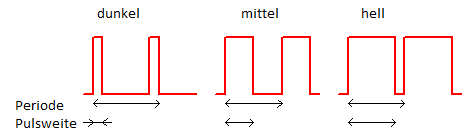
\includegraphics[width=0.8\textwidth]{skizzen/pwm.png}
  \end{center}
  \caption{Schema der Pulsweitenmodulation}
  \label{pwm_schma}
\end{figure}



	\section{Betrachtung der Komponenten}
\subsection{Mikrocontroller}
Die zentrale Komponente der Digitaluhr ist der Mikrocontroller ATmega32. Der von Atmel hergestellte 8-bit Kontroller ist im 40-pin DIP Format verfügbar. Dies ermöglicht die einfache Verwendung auf einer Lochrasterplatine mit 2,54mm Lochabstand. Programmiert wird der ATMega entweder in C oder in AVR-Assembler, die Wahl fiel hier auf die konfortablere Sprache C.
Viele der integrierten Komponenten wurden genutzt: Das zur Verfügung gestellte SPI-Interface \footnote{Serial Peripheral Interface Bus}zur Kommunitkation mit den Schieberegistern, der integrierte AD-Wandler zur Auswertung des Helligkeitssensors, das ISP-Interface zur Programmierung. TODO: Gibts hier noch mehr?
\begin{table}[htp]
  \centering
  \renewcommand{\arraystretch}{1.2}
  \begin{tabular}{||l | l||}
  \hline\hline
  Bezeichnung&ATMEGA32 16PU 0926D\\\hline
  Hersteller&Atmel\\\hline
  Architektur&AVR 8-bit \\\hline
  Geschwindigkeit&bis 16Mhz \\\hline
  Programmspeicher&32 KiB Flash \\\hline
  Arbeitsspeicher&2 KiB SRAM \\\hline
  EEPROM&1 KiB \\\hline
  AD-Wandler&8 Kanal / 10 Bit \\\hline
  Bauform&40-pin DIP Gehäuse \\
  \hline\hline    
\end{tabular}
\caption{Eckdaten des ATmega 32}
\end{table}

\subsection{DCF77 Empfangsmodul}\label{sec_dcf77modul}
Das in der Digitaluhr verwendete Modul ist die \glqq C-Control DCF-Empfängerplatine\qrqq\footnote{\url{http://www.conrad.de/ce/de/product/641138/C-Control-DCF-Empfaengerplatine}, Bestellnummer: 641138 - 62}~ (siehe Abbildung \ref{fig_dcf77}) von Conrad.

\begin{center}
\setlength{\fboxsep}{0pt}
\fbox{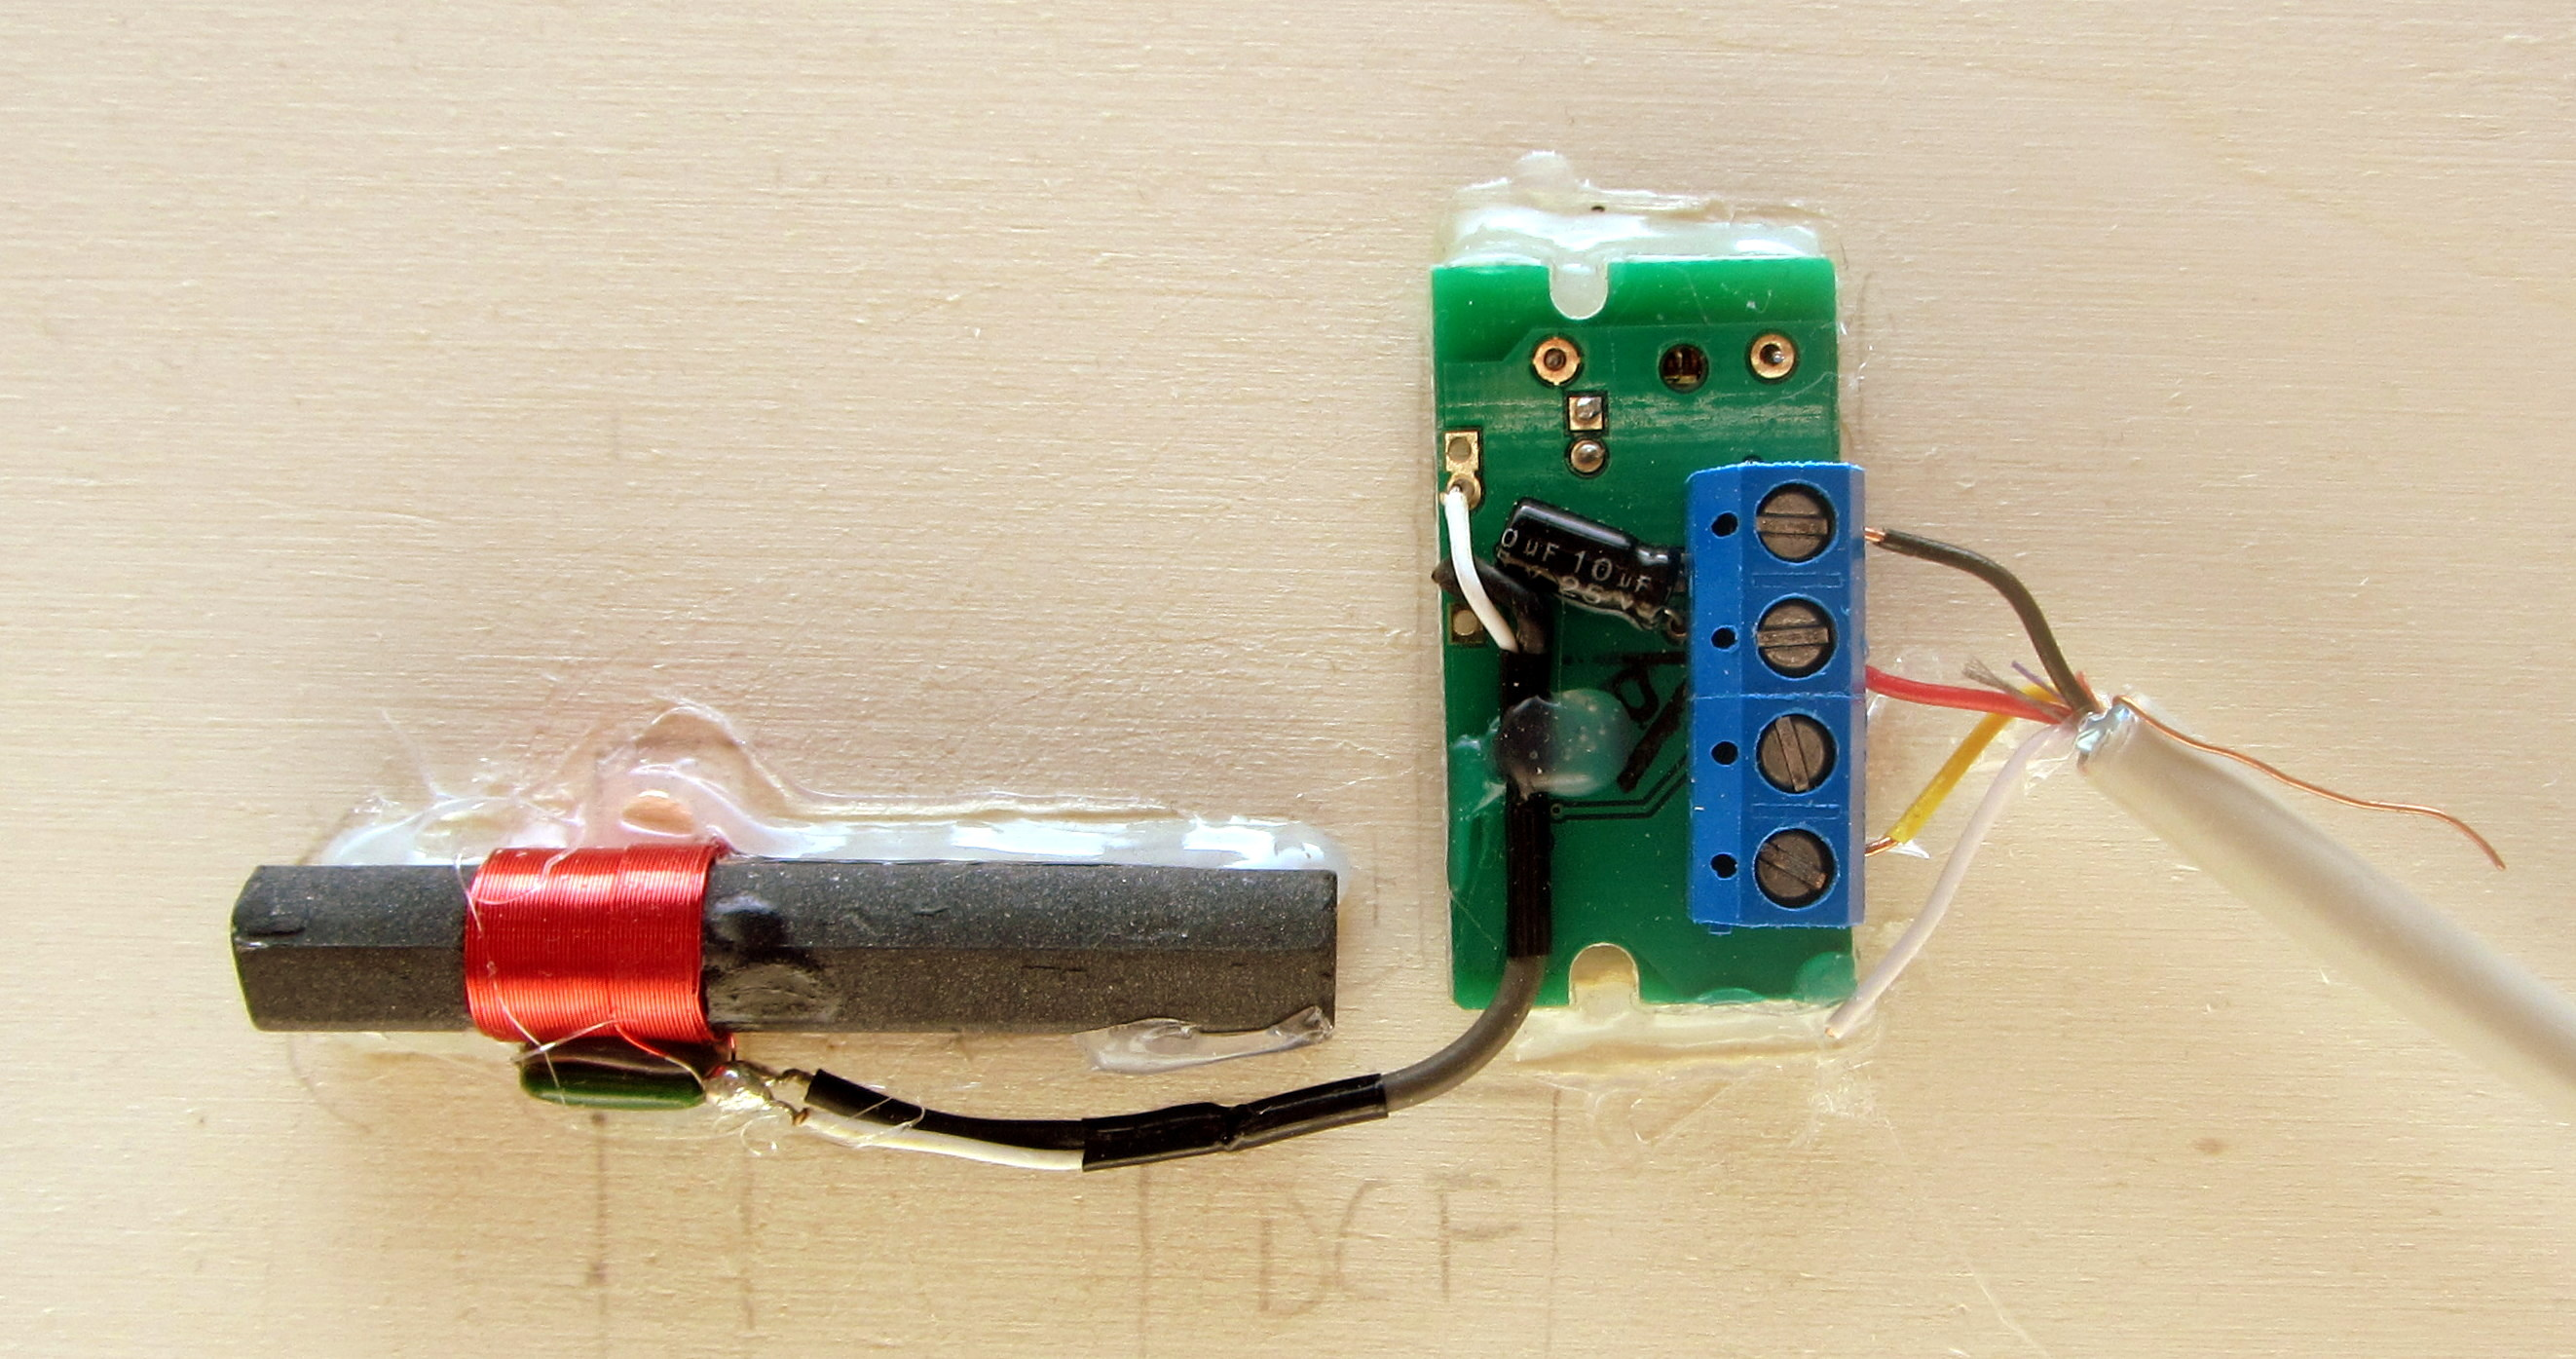
\includegraphics[width=0.75\textwidth]{images/dcf_empfaenger.jpg}}
\captionof{figure}{C-Control-DCF-Empfängerplatine von Conrad}\label{fig_dcf77}
\end{center}
%
% \begin{figure}[h]
%   \begin{center}
%   \begin{minipage}[c]{0.5\textwidth}
%         \fbox{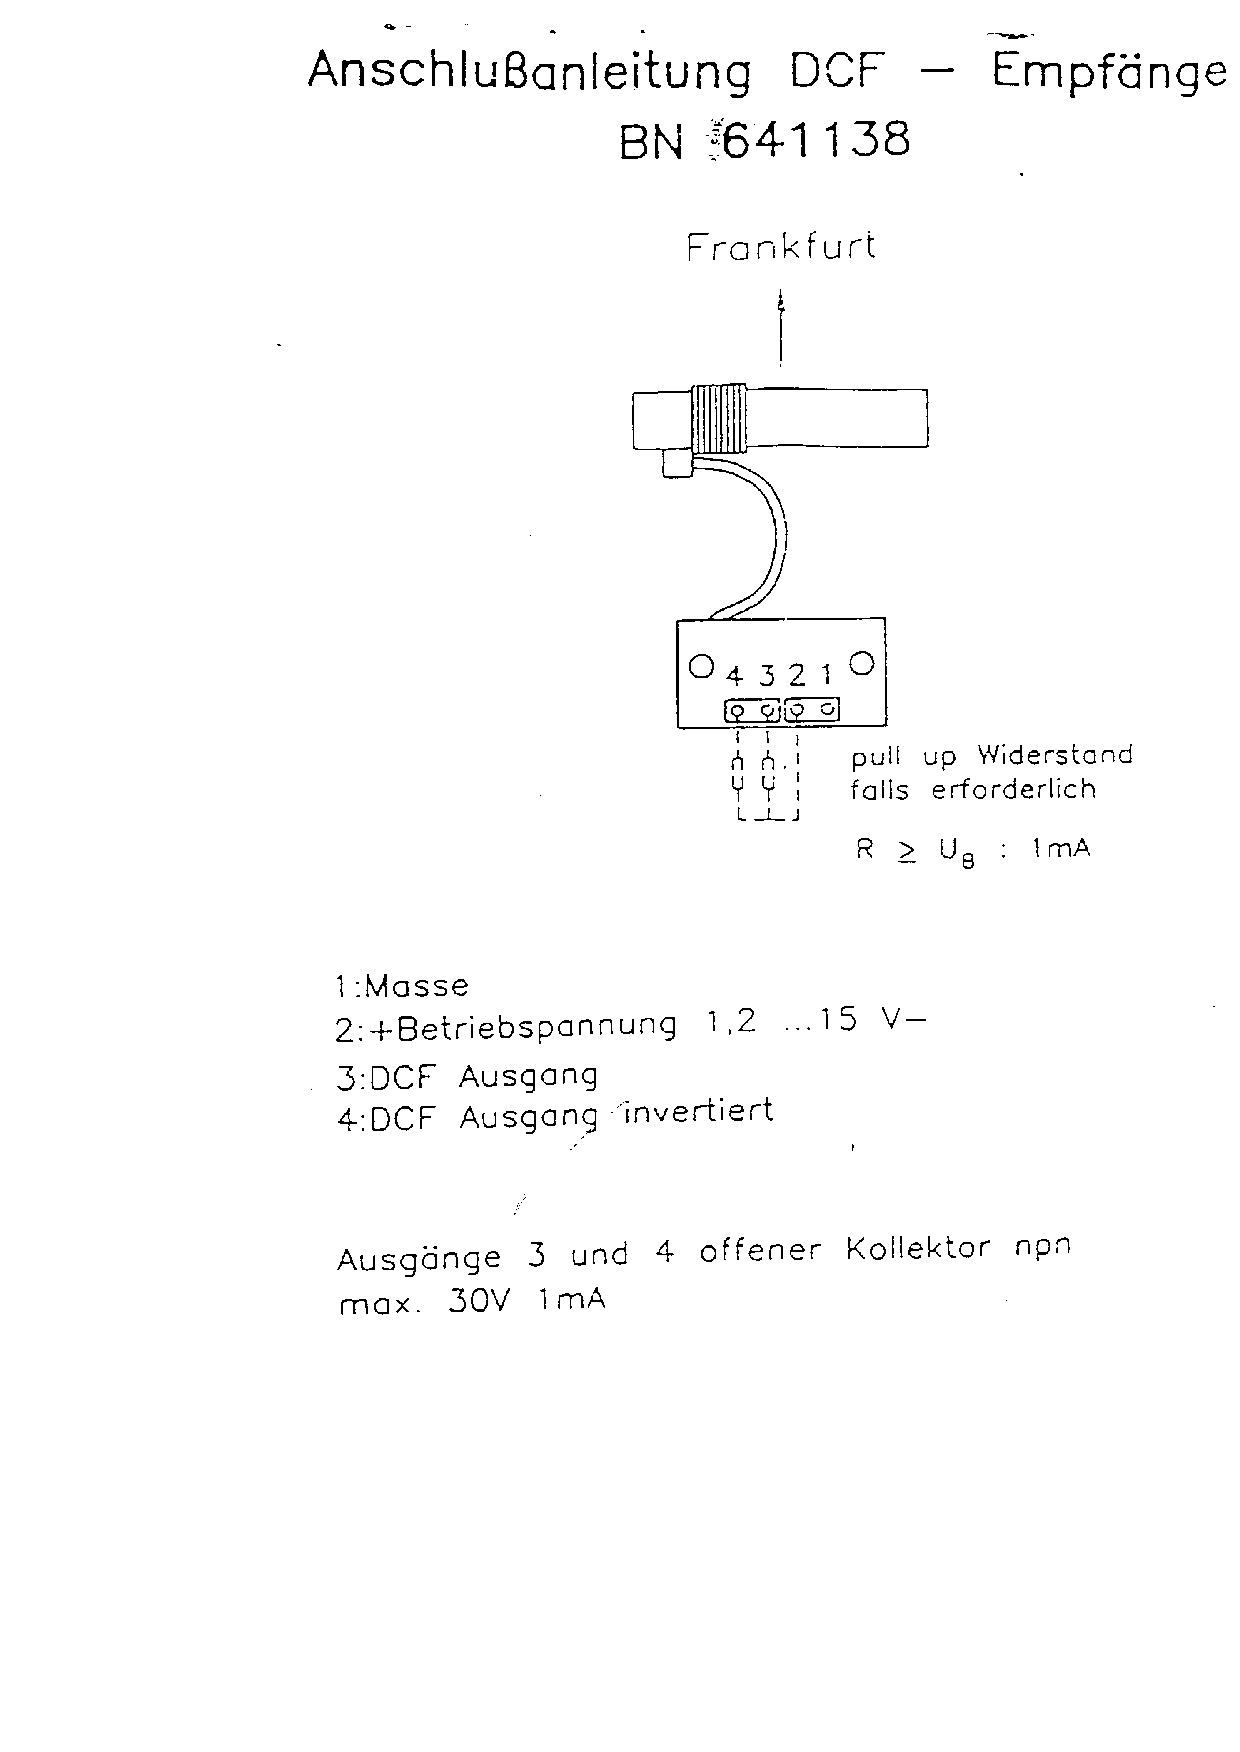
\includegraphics[width=\textwidth]{Literatur/conrad_dcf77.pdf}}
%         \caption{Anschlussanleitung DCF77 Modul\footnotemark}
%   \end{minipage}
%   \hspace{0.07\textwidth}
%   \begin{minipage}[c]{0.4\textwidth}
% Das Modul besitzt 4 Anschlüsse, welche im Anschlussplan links beschrieben sind. Es wird der \texttt{DCF Ausgang invertiert} für das Datensignal verwendet. Er ist an Microcontrollerpin PB2 angeschlossen. Damit die Uhrzeit auf jeden Fall richtig empfangen wird, ist einerseits die Ausrichtung Richtung Frankfurt wichtig sowie andererseits die Verwendung eines fehlertoleranten Codes zur Auswertung der Uhrzeit. Außerdem sollte darauf geachtet werden, das Modul nicht zu nah an Störquellen zu stellen. Als starke Störquelle stellten sich bei der Entwicklung Monitore heraus. In Abbildung TODO ist der Unterschied zwischen einem einwandfreien Signal und einem, durch einen Monitor in 2m Entfernung, gestörtem Signal abgebildet. Es ist zu erkennen, dass das Signal plötzlich im Mikrosekundenbereich gleichmäßig alterniert, also von dem ursprünglichen Signal nichts mehr zu erkennen ist.
%   \end{minipage}
%   \end{center}
% \end{figure}
%\addtocounter{footnote}{-1}%
%\footnotetext{Quelle: \url{http://www.produktinfo.conrad.com/datenblaetter/625000-649999/641138-an-01-de-Anschlussplan_DCF_Empfaengerplatine.pdf}}%
%\stepcounter{footnote}%
%

\begin{wrapfigure}{r}{0.50\textwidth}
  \vspace{-25pt}
  \begin{center}
    \fbox{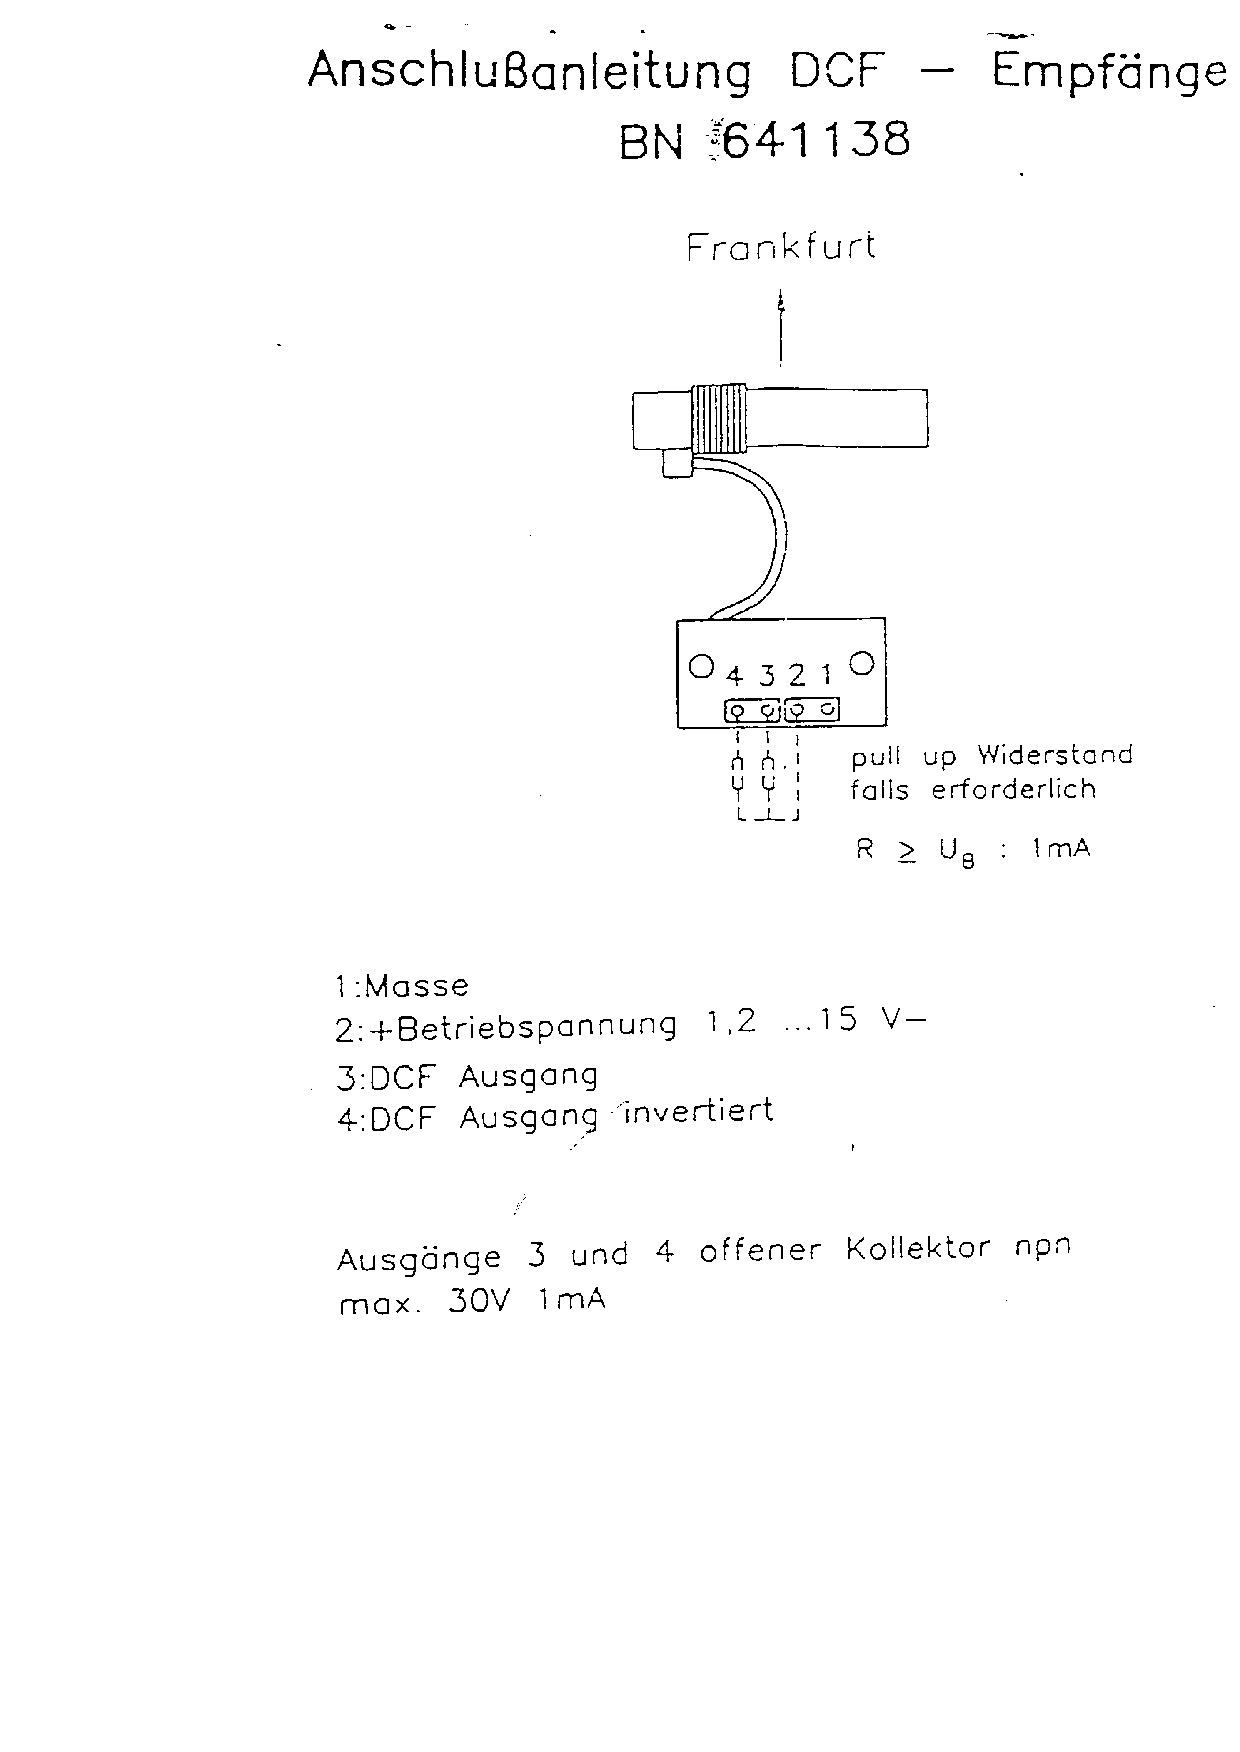
\includegraphics[width=0.45\textwidth]{Literatur/conrad_dcf77.pdf}}
  \end{center}
  \vspace{-20pt}
  \captionof{figure}{Anschlussanleitung DCF77 Modul\footnote{Quelle: \url{http://www.produktinfo.conrad.com/datenblaetter/625000-649999/641138-an-01-de-Anschlussplan_DCF_Empfaengerplatine.pdf}}}
\end{wrapfigure}
%
Das Modul besitzt 4 Anschlüsse, welche im Anschlussplan links beschrieben sind. Es wird der \texttt{DCF Ausgang invertiert} für das Datensignal verwendet. Er ist an Microcontrollerpin PB2 angeschlossen. Damit die Uhrzeit auf jeden Fall richtig empfangen wird, ist einerseits die Ausrichtung Richtung Frankfurt wichtig sowie andererseits die Verwendung eines fehlertoleranten Codes zur Auswertung der Uhrzeit. Außerdem sollte darauf geachtet werden, das Modul nicht zu nah an Störquellen zu stellen. Als starke Störquelle stellten sich bei der Entwicklung Monitore heraus. In Abbildung TODO ist der Unterschied zwischen einem einwandfreien Signal und einem, durch einen Monitor in 2 m Entfernung, gestörtem Signal abgebildet. Es ist zu erkennen, dass das Signal plötzlich im Mikrosekundenbereich gleichmäßig alterniert, also von dem ursprünglichen Signal nichts mehr zu erkennen ist.

Nachfolgend soll die Funktion \texttt{byte conrad\_state\_get\_dcf\_data()} erklärt werden. Diese Funktion ist für den Empfang der Daten des DCF77 Moduls verantwortlich. Sie als State Machine realisiert und wird beim Empfangen der Daten jede 10 ms aufgerufen. Dies wird gemacht, weil die Funktion sonst sehr lange laufen würde (der vollständige Empfang der Daten dauert im Best Case 60 Sekunden) und andere Funktionen ihre Arbeit nicht mehr verrichten können. Mit diesem Ansatz aber bleibt die Uhr reaktiv und kann beispielsweise weiterhin auf Tasterevents reagieren.
%
\begin{lstlisting}[language=C,label=dcf_state_data1,caption=Empfang des DCF77 Signals - Minutenstart erkennen]
if (i < 155) {
    /* DCF Signal unmoduliert (da es invertiert ist, ist es standartmaessig 1) */
    if (DCF_VALUE != 0) {
        i++;
        j = 0;
        DBG_LED_OFF();
    /* Wenn es moduliert ist (logisch 0) */
    } else {
        j++;

        if (j > 7) {
            i = 0;
            j = 0;
            DBG_LED_ON();
        }
    }
    return T2_WAIT;
}
\end{lstlisting}
%
In Listing \ref{dcf_state_data1} ist zunächst der erste Teil der Funktion zu sehen. Dabei geht es um das Erkennen des Minutenanfangs. Wie im DCF77 Grundlagenkapitel \ref{sec_dcfgrund} erläutert, wird das Signal beim übergang von der 59. auf die 60. Sekunde nicht moduliert, es muss also 2 Sekunden unmoduliert sein.

Die Variable i zählt die Zentisekunden, in denen das Signal unmoduliert ist. Aus Toleranzgründen wird lediglich geschaut, ob i den Wert von 155 übersteigt, statt 200 (= 2 s). Es kann nämlich passieren, dass das Signal zufällig genau zum Messzeitpunkt leicht abfällt. Deshalb werden auch Werte von j, welches die modulierten Zentisekunden misst, von weniger als 70 ms ignoriert. Somit werden Ungenauigkeiten durch, die durch Tests ermittelten, Werte von 155 und 7 ziemlich zuverlässig vermieden.

Wie zu erkennen ist, gibt es keine Schleife, sondern lediglich sequentiellen Code, der auf jeden Fall returned (siehe Zeile 17). Es gibt die folgenden Return-Codes:
%\begin{description}
%\item[T2\_WAIT] Resettet den Counter von Timer2, sodass genau 10 ms gewartet wird
%\item[ERROR] Bricht den Messvorgang ab, weil ein Fehler aufgetreten ist
%\item[SUCCESS] Alle 60 Bits wurden gemessen. Dabei wurde kein Fehler erkannt
%\end{description}
%
\begin{list}{\ding{42}}
{\setlength{\topsep}{0cm}
\setlength{\itemsep}{0.2cm}
\setlength{\leftmargin}{3cm}
\setlength{\labelwidth}{3cm}
\setlength{\labelsep}{0cm}
\renewcommand{\makelabel}[1]{\textbf{\textsf{\normalsize #1} }}}
\item[T2\_WAIT] Resettet den Counter von Timer2, sodass genau 10 ms gewartet wird
\item[ERROR] Bricht den Messvorgang ab, weil ein Fehler aufgetreten ist
\item[SUCCESS] Alle 60 Bits wurden gemessen. Dabei wurde kein Fehler erkannt
\end{list}
%
%\lstinputlisting[label=samplecode,caption=A sample]{sourceCode/HelloWorld.java}
%
%
In diesem Fall wird der Returncode \texttt{T2\_WAIT} verwendet, damit die Funktion nach 10 ms nochmals aufgerufen wird und die Messung fortgesetzt werden kann.
%
\begin{lstlisting}[language=C,label=dcf_state_data2,caption=Empfang des DCF77 Signals - Sekunde analysieren]
if (is_start_of_sec) {
    /* Pausiere bis zum modulierten Signal */
    if (DCF_VALUE != 0) {
        return T2_WAIT;
    }
    is_start_of_sec = false;
}
if (k < 95) {
    if (DCF_VALUE != 0) {
        unmodulated++;
    } else {
        if (k < 40) {
            modulated++;
        }
    }
    k++;
    return T2_WAIT;
}
\end{lstlisting}
%
Der nächste Schritt (siehe Listing \ref{dcf_state_data2}) ist das Analysieren jeder Sekunde, also das Zählen der modulierten und nicht-modulierten Signale. Dazu wird zunächst gewartet, bis die Sekunde anfängt, also das erste modulierte Signal auftritt (Zeile 3), anschließend wird 95 \% der Sekunde analysiert. Die letzten 5 \% sind Toleranz, damit die nächste Sekunde sicher erkannt werden kann. Modulierte Signale treten nur in den ersten 200 ms einer Sekunde auf, deshalb werden sie nur am Anfang gezählt, aber aus Toleranzgründen innerhalb der ersten 400 ms (Zeile 12). Auch hier wird nach jeder Messung die Routine mit \texttt{T2\_WAIT} verlassen (Zeile 17).
%
\begin{lstlisting}[language=C,label=dcf_state_data3,caption=Empfang des DCF77 Signals - Sekunde analysieren]
if (unmodulated > 50 && unmodulated < 140) {
    /* Wenn moduliert zwischen 50 und 140 ms, liegt logisch 0 an */
    if (modulated > 5 && modulated < 14) {
        dcf_data[secs] = 0;
    /* Zwischen 150 ms und 240 ms, liegt logisch 1 an */
    } else if (modulated > 15 && modulated < 24) {
        dcf_data[secs] = 1;
    /* sonst ist es ungueltig */
    } else {
        return ERROR;
    }
} else {
    return ERROR;
}
/* Bereite die naechste Sekunde vor */
secs++;
is_start_of_sec = true;
k = 0;
modulated = 0;
unmodulated = 0;

return SUCCESS;
\end{lstlisting}
%
Als letztes werden die Daten ausgewertet, also geprüft ob logisch eine 0 oder 1 gemessen wurde. Dazu wurden Zahlen gewählt, die sich durch Tests bewährt haben (siehe Listing \ref{dcf_state_data3}). Bei fehlerhaften Daten wird \texttt{ERROR} zurückgegeben (Zeile 10 und 13) und die gesamte Messung abgebrochen. Sind die Daten gültig, wird die State Machine auf den Anfangszustand jeder Sekunde gesetzt (Zeilen 16 -- 20) und \texttt{SUCCESS} zurückgegeben und damit die Auswertung der nächsten Sekunde begonnen.

Wie zu sehen ist, werden statt diskreten Werten immer Bereiche angenommen, in denen ein bestimmter Wert liegen muss. Dies ist durch die funkbedingten Ungenauigkeiten unbedingt notwendig. Es erforderte einige Tests, bis die passenden Werte gefunden wurden, um einen passablen Empfang zu erreichen, was letzten Endens jedoch gelang und zu einem korrekt funktionierendem Funkmodul für die Digitaluhr führte.
%
\subsection{LED Matrix}
\subsubsection{Schaltung und Hardware}
\begin{center}
	\includegraphics[width=\textwidth]{images/LED_Matrix.png}
	\captionof{figure}{LED Matrix Draufsicht}
\label{led_oben}
\end{center}
Die LED Matrix dient der Uhr als Display. Es werden $7*17=119$ blaue
LEDs\footnote{LED Spexx TODO} verwendet. Die LEDs haben einen Abstand von $45 mm$ und werden durch ein Gitter aus Sperrholz voneinander getrennt, so dass
Pixel entstehen. Durch das Multiplexen der Zeilen kann jede LED unabhängig
gesteuert werden.

Die Anoden der Reihen sind jeweils verbunden und an die Schieberegister TODO REF
angeschlossen. Die Kathoden sind Zeilen verbunden und über die Mosfets vom
Mikrocontroller geschaltet. Eine Ausnahme bildet Reihe 17, da die 2
Schieberegister nur 16 Ausgänge bieten wurde diese direkt an den Mikrocontroller
angeschlossen.
\begin{center}
	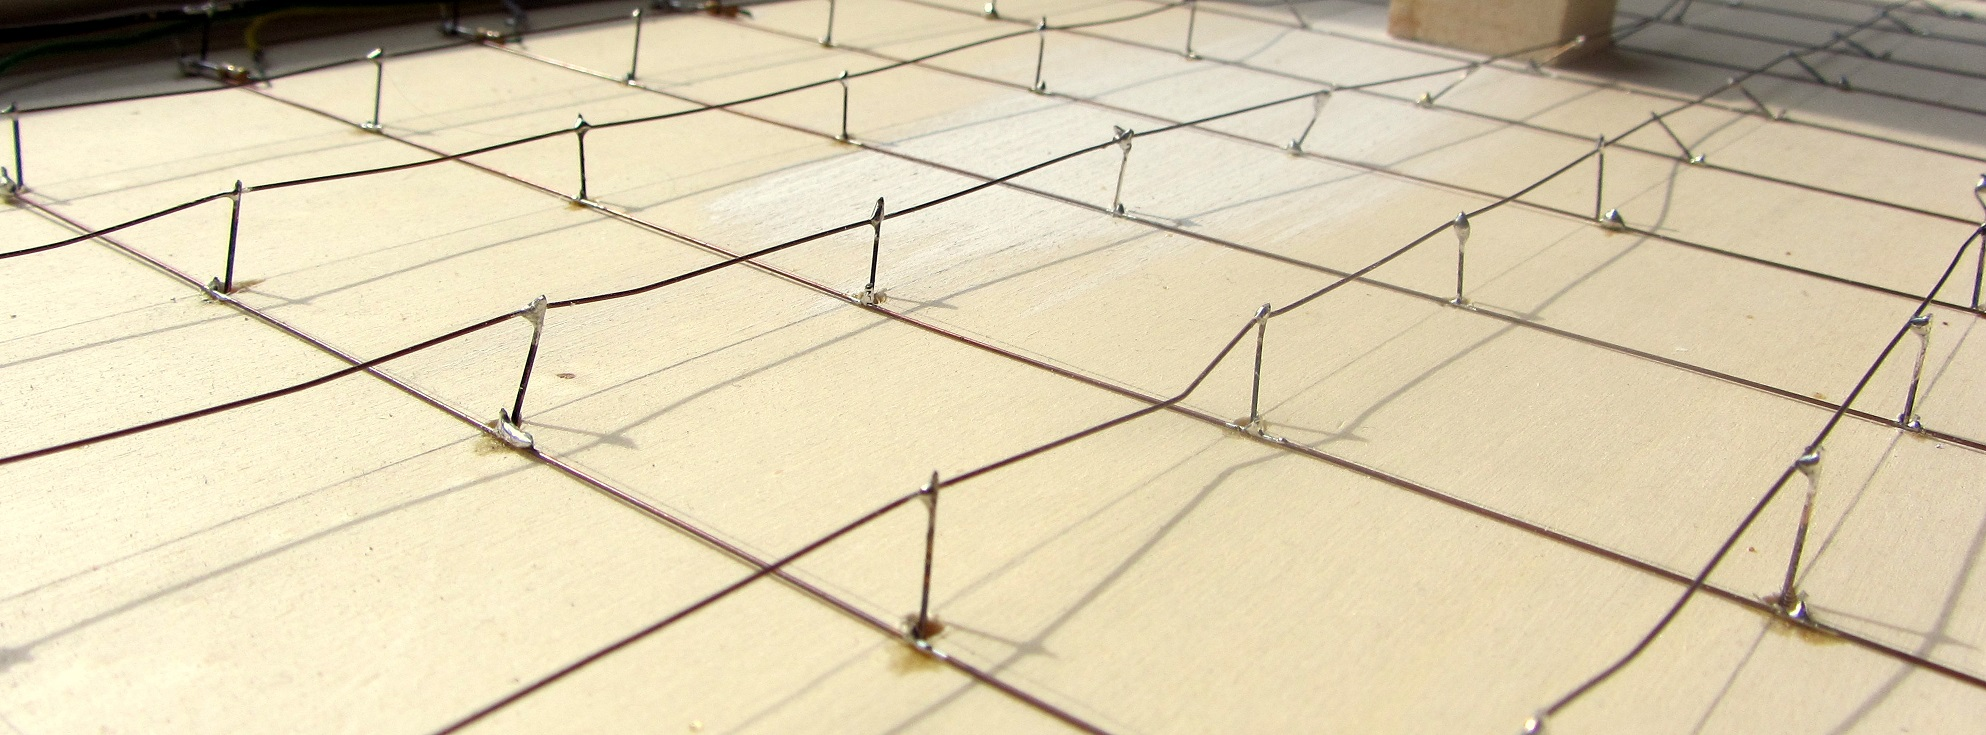
\includegraphics[width=\textwidth]{images/unterseite_drahtgitter.jpg} 
\captionof{figure}{LED Matrix Verdrahtung, Anoden aufliegend und Kathoden
schwebend verbunden}
\end{center}
\label{led_matrix_verdrahtung}

\begin{center}
	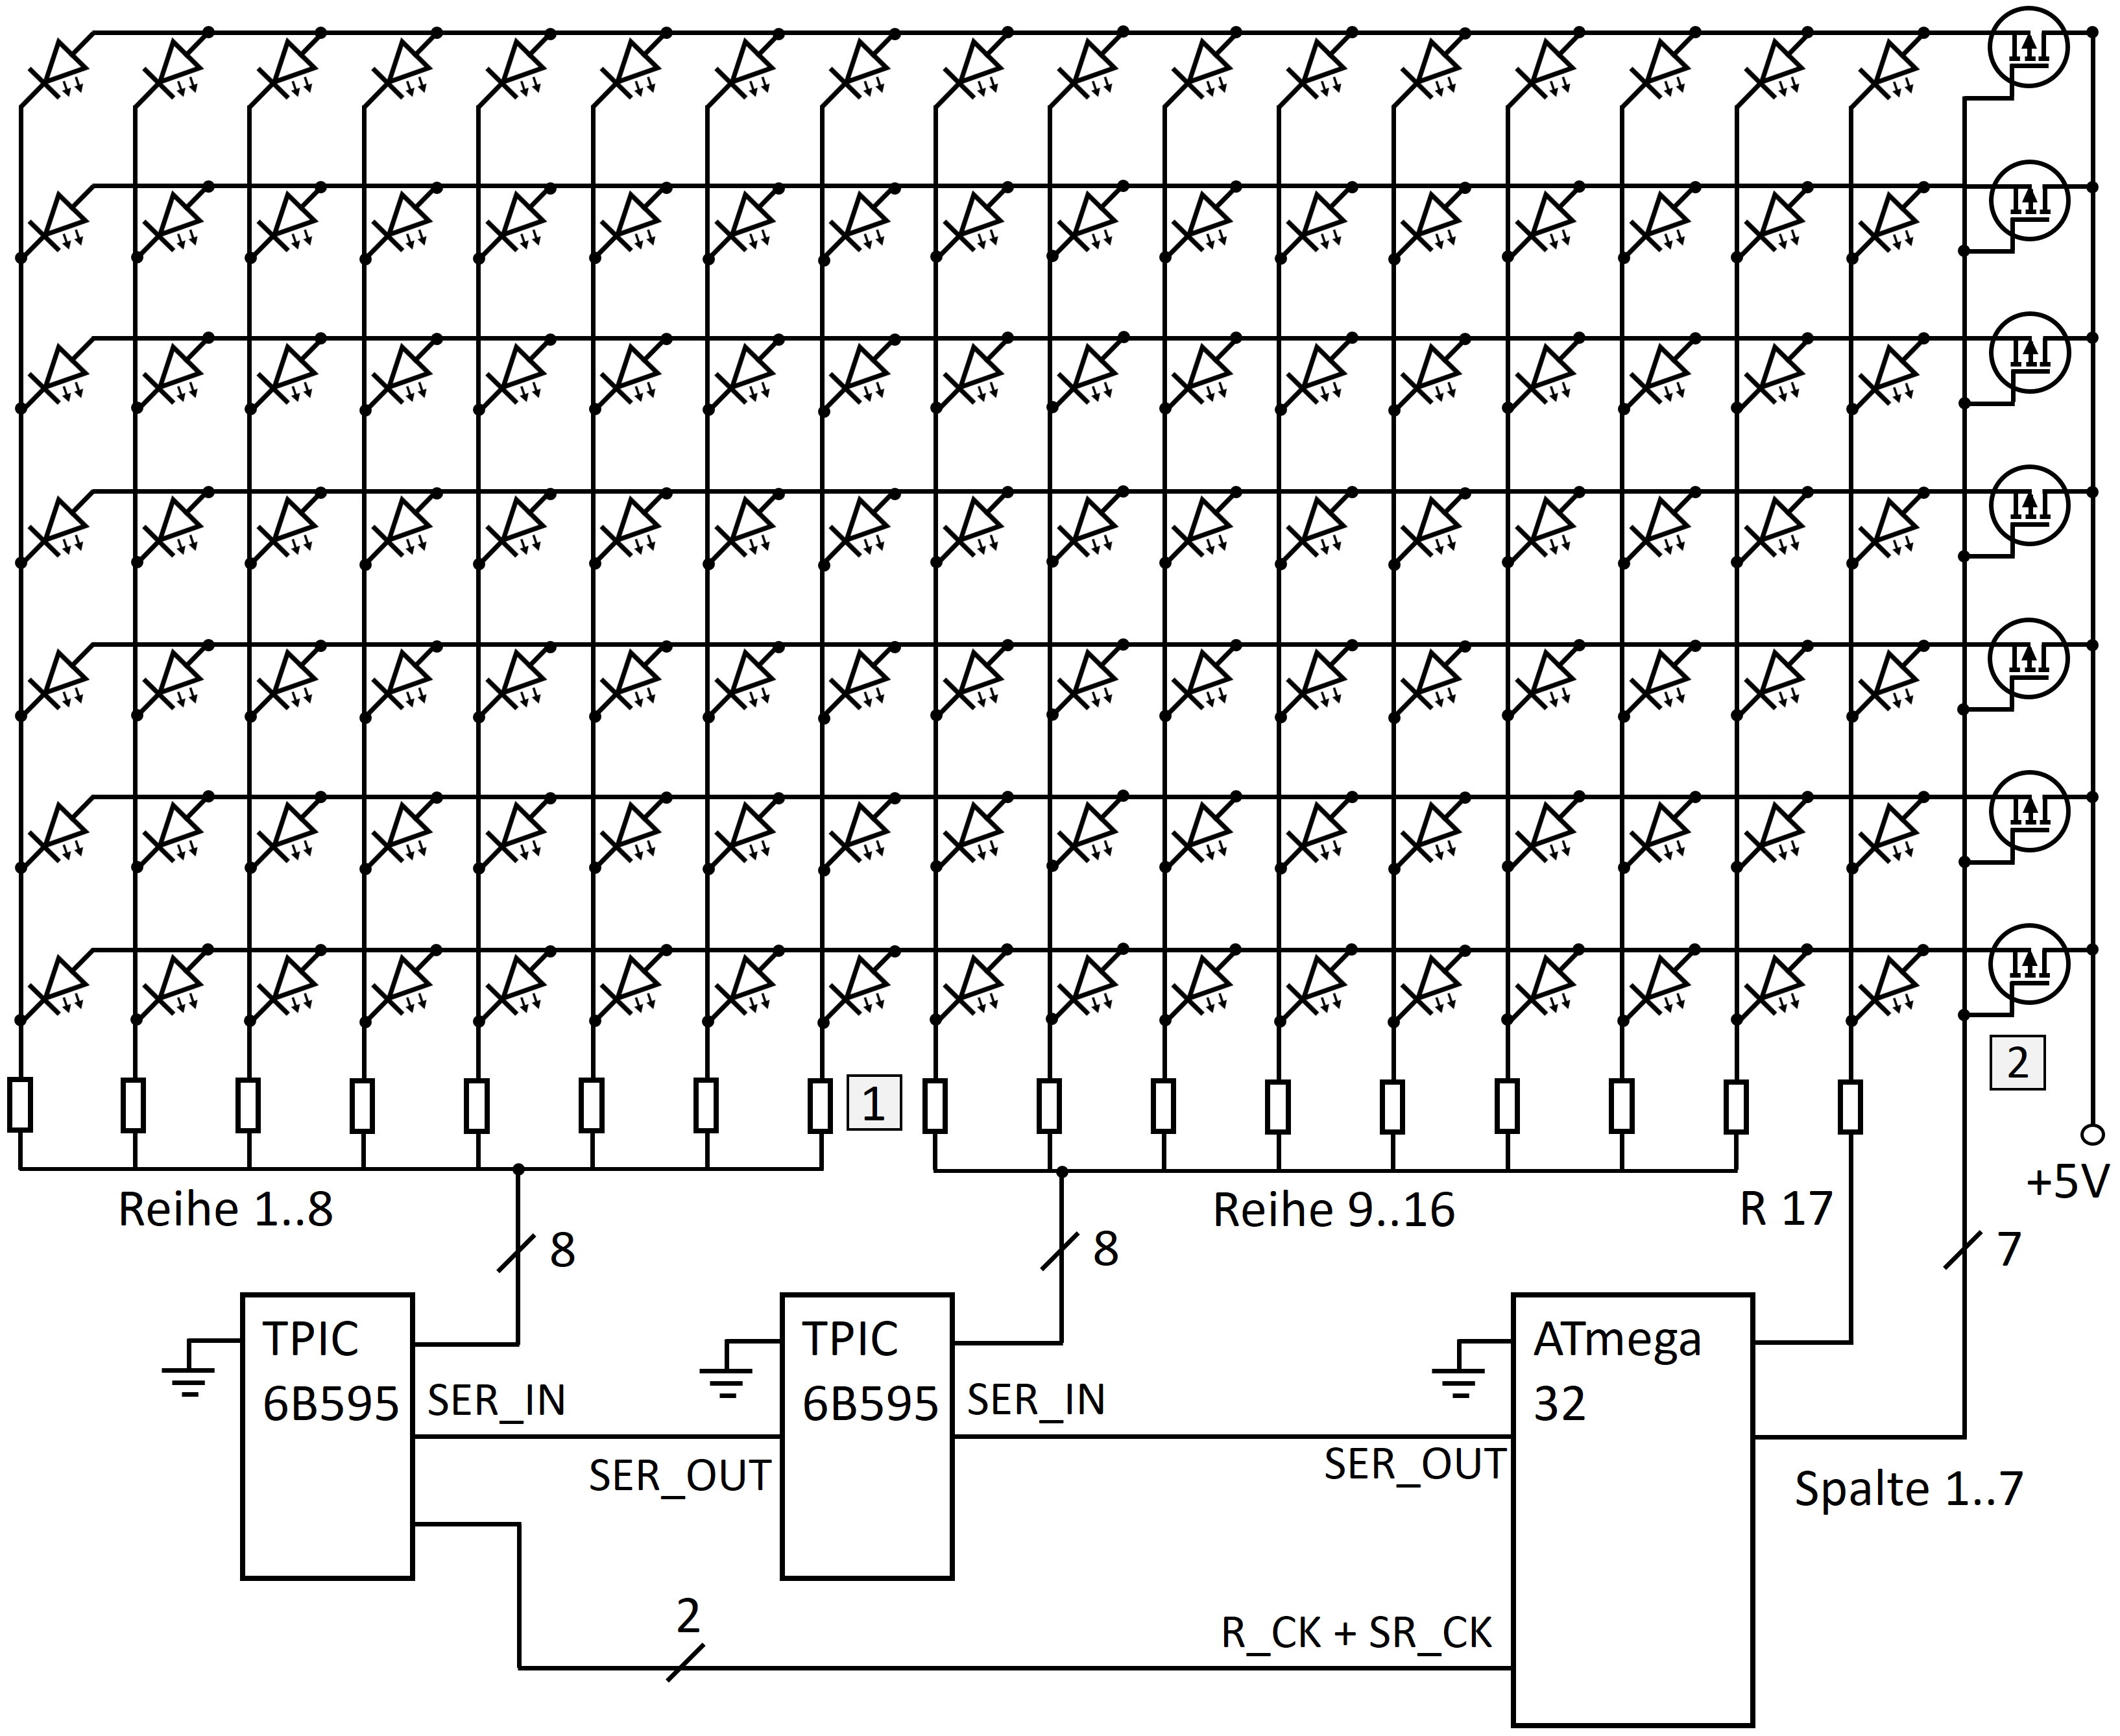
\includegraphics[width=\textwidth]{skizzen/led_matrix_schaltplan.png} 
\captionof{figure}{LED Matrix Schaltplan, 1: LED
Vorwiderstände, 2: P-Kanal Mosfets \mbox{IRLZ24N}}
\end{center}
\label{led_matrix_schaltplan}

Durch die Ansteuerung als Matrix werden nur 24 Leitung von der LED Anzeige zur
Hauptplatine benötigt. Da der Mikrocontroller auf seinen Logikausgängen nicht
die benötigte Leistung bereitstellen kann wird die Spannung durch die P-Kanal
Mosfets vom Typen IRLZ24N geschalten.

Um weitere Pins am ATmega einzusparen werden die Reihen (abgesehen von Reihe 17)
mittels Schieberegister gesteuert. Die beiden Schieberegister vom Typen
TPIC6B595 können dauerhaft Ströme bis zu 150mA pro Pin und 500mA Gesamtstrom gegen GND
schalten.\footnote{vgl. \cite{6b595}, S. 1} Die Kommunikation zwischen ATmega
und den Schieberegistern erfolgt über das SPI Interface, welches sehr einfach mit Daten gefüllt werden kann und
diese unabhänig vom eigentlichen Programmablauf an die Schieberegister schickt.

\begin{wrapfigure}{r}{0.5\textwidth}
  \vspace{-25pt}
  \begin{center}
    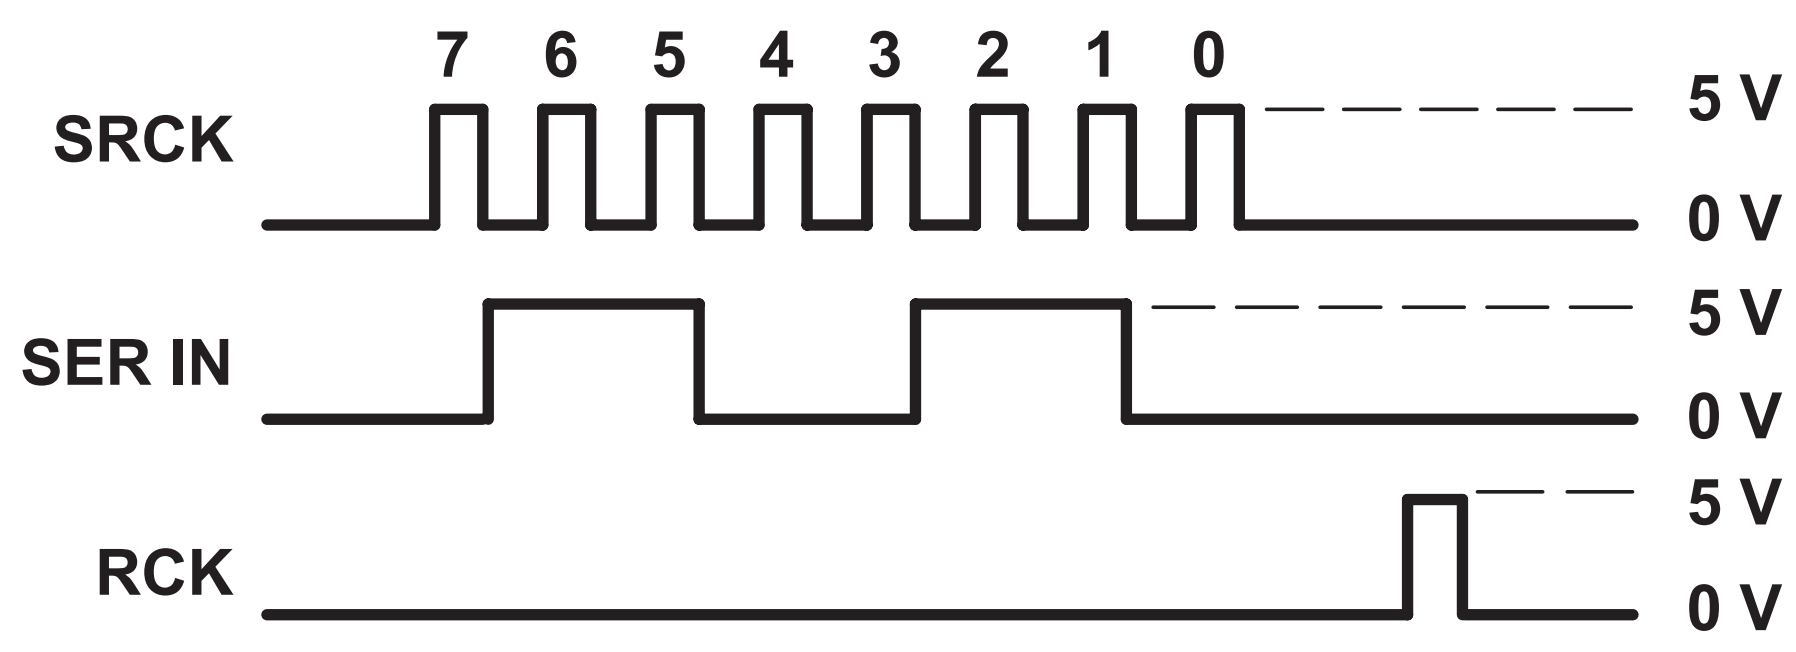
\includegraphics[width=0.48\textwidth]{skizzen/schieberegister_linien.png}
  \end{center}
  \vspace{-20pt}
  \captionof{figure}{Füllen des Schieberegisters\footnote{\cite{6b595}, S. 5}}
\end{wrapfigure}

Das SPI Interface wird über 3 Leitungen realisiert: SER IN als Datenleitung,
SRCK zur Taktübertragung, RCK um die Daten vom Schieberegister auf die
Ausgänge zu legen. Das zweite Schieberegister wird parallel an RCK und SRCK
verbunden, und der serielle Ausgang des ersten Schieberegisters SER OUT wird mit
SER IN des zweiten Schieberegister verbunden, durch diese Schaltung erreicht man
quasi ein 16-bittiges Schieberegister.
Insgesamt benötigt das Display somit 11 Pins am Mikrocontroller: 3 für die
Schieberegisteransteuerung, 7 für die Ansteuerung der Mosfets sowie eine Leitung
um Reihe 17 zu schalten.
\subsubsection{Software}

\subsection{Helligkeitssensor}
Ein Fotoresitor (Lichtabhängier Widerstand, kurz LDR für Light Dependend Resistor) bildet einen Teil eines Spannugteilers. Die innerhalb des Spanungsteilers anliegende Spannung wird dann vom Mikrocontroller mit Hilfe des AD-Wandlers ausgewertet.
Der verwendete Fotoresisor besitzt nominal einen Dunkelwiderstand von $100 k\Omega$ .
Um den Widerstandsverlauf besser abschätzen zu können wurden Messungen vorgenommen.
\begin{figure}[h]
  \begin{center}
  \begin{minipage}[b]{0.3\textwidth}
        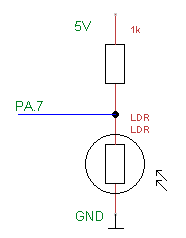
\includegraphics[height=4.5cm]{skizzen/helligkeitssensor_schmatic.png}
        \caption{Spannungsteiler des LDRs}
  \end{minipage}
  \hspace{0.07\textwidth} 
  \begin{minipage}[b]{0.6\textwidth}
    \begin{tabular}[h]{||l | l||}
	  \hline \hline
	  Dunkelheit& $70 k\Omega$ \\ \hline
	  Zimmerhelligkeit & $3 k\Omega$ \\ \hline
	  Schreibtischlampe 50cm Abstand& $500 \Omega$ \\ \hline
	  Schreibtischlampe 10cm Abstand& $90 \Omega$ \\ \hline
	  Schreibtischlampe 2cm Abstand& $30 \Omega$  \\
	  \hline\hline
    \end{tabular} 
    \label{Modellversuch} 
    \captionof{table}{Widerstandmessung des LDR}
  \end{minipage}
  \end{center}
\end{figure}
%
\subsection{Temperatursensor}
Als Temperatursensor wurde der DS18S20\footnote{\url{http://www.maximintegrated.com/datasheet/index.mvp/id/2815}} von Maxim Integrated verwendet. Dieser verwendet das 1-Wire\textsuperscript{\textregistered}-Protokoll\footnote{\url{http://www.maximintegrated.com/products/1-wire/flash/overview/index.cfm}}, sodass nur ein Datenpin vonnöten ist, worüber Befehle gesendet sowie Daten empfangen werden.

Der 1-Wire-Bus ermöglicht die Verwendung mehrerer Geräte an der Datenleitung, wobei jedes Gerät über seine eindeutige 64-Bit ID angesprochen wird. Da bei diesem Projekt lediglich ein DS18S20 verwendet wird, kann die Ansteuerung der eindeutigen ID weggelassen werden und alle Geräte auf dem Bus angesprochen werden, da keine Kollision entstehen kann.

Der Temperatursensor wird wie in Grafik \ref{fig_tempsensor} angeschlossen. Die Datenleitung wird über einen $4,7 k\Omega$ Pullup-Widerstand mit der Spannungsquelle verbunden, sowie an Pin PA6 des Microcontrollers angeschlossen.
%
\begin{figure}[htp]
\centering
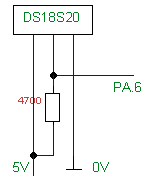
\includegraphics{skizzen/temperatursensor_schematic.png}
\caption{Schaltung für den 1-Wire Temperatursensor}\label{fig_tempsensor}
\end{figure}
%
Für das 1-Wire-Protokoll ist ein genaues Timing unabdingbar, deshalb müssen bei jeglicher Kommunikation mit dem DS18S20 alle Interrupts ausgeschaltet werden. Da die längste Kommunikation am Stück der Reset-Pulse mit $960 \mu s$ ist, ist das Auschalten der Interrupts für die Funktionalität der Uhr nicht beeinträchtigend.

Das Protokoll sieht vor, dass jede Kommunikation mit einem Reset-Pulse startet. In Abbildung \ref{fig_resettiming} 
ist das genaue Timing des Reset-Pulses zu erkennen. Zunächst muss der Master, also hier der Microcontroller den Bus für mindestens $480 \mu s$ auf Low ziehen. Nach Freigabe des Busses sorgt der Pullup-Widerstand dafür, dass der Bus wieder auf High gesetzt wird. Anschließend zieht der Sensor den Bus nach $15 \mu s$ bis $60 \mu s$ nach der ansteigenden Flanke für $60 \mu s$ bis $240 \mu s$ auf Low. Dies signalisiert dem Master, dass ein Gerät am Bus hängt und einsatzbereit ist.\footnote{\cite{ds18s20}, Seite 13}

In der weiteren Kommunikation wird nun das \texttt{SKIP ROM} Kommando benutzt, welches bedeutet, dass die 64-Bit ID weggelassen werden kann und alle Geräte (hier nur eins) angesprochen werden. Nun kann der DS18S20 mit dem \texttt{CONVERT TEMP} Kommando dazu aufgefordert werden, die Temperatur zu messen und digital zu konvertieren. Dies macht er nicht permament um Strom zu sparen. Nach einer Konvertierungszeit von mindestens $700 ms$ kann die Temperatur ausgelesen werden. Dazu muss erneut ein Reset- sowie ein Skiprom-Kommando gesendet werden, um dann mit \texttt{READ SCRATCHPAD} die eigentliche Temperatur zu erhalten.\footnote{Genaue Beschreibung der Kommandos siehe \cite{ds18s20} Seite 10ff}
%
\begin{figure}[htp]
\centering
\centerline{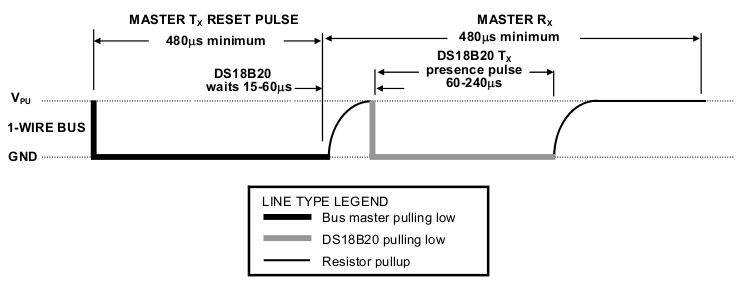
\includegraphics[width=\linewidth]{skizzen/temperatur_reset.png}}
\caption{Reset-Pulse Timing Diagramm\footnote{\cite{ds18s20}, Seite 13}}\label{fig_resettiming}
\end{figure}
%
\subsection{Gehäuse}
%TODO
%
Ziel war es ein optisch ansprechendes, sowie funktionales Gehäuse zu kreieren. 

Als problematisch stellte sich die Zielsetzung der flachen Bauart heraus. Denn um eine gleichmässige Lichtverteilung innerhalb eines Pixels zu erreichen, muss ein relativ großer Abstand zur LED gegeben sein. Durch praktisches Testen ergab sich für die verwendeten LEDs ein idealer Abstand von .%TODO eventuell wirklich probieren 
Außerdem muss verhindert werden, dass die offenliegende Verdrahtung der LED-Matrix zu Kurzschlüssen führt. Im Besonderen ist hier das Netzteil zu nennen, da hier ein Spannung von 230 Volt anliegt und das Netzteil von allen Komponenten mit 15 mm %TODO 
über die höchste Bauhöhe verfügt. 
Die Bauhöhe der Verdrahtung der LED-Matrix wurde an den kritischen Stellen von 5 -- 6 mm auf ca. 2 mm verringert. Um Kurzschlüsse innerhalb der LED-Matrix zu verhindern, wurden die Kreuzungspunkte zum Teil isoliert.
\begin{center}
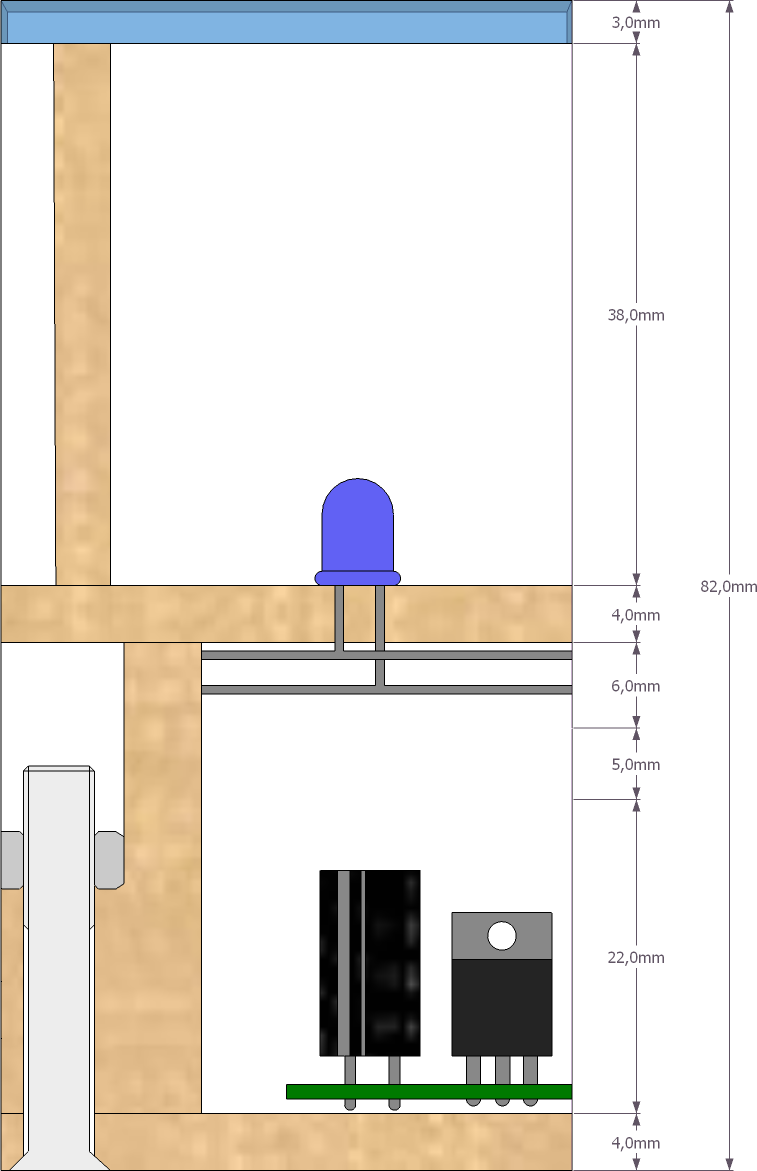
\includegraphics[width=0.6\textwidth]{skizzen/querschnitt.png}
\captionof{figure}{Schematischer Querschnitt des Gehäuses}
\label{fig_querschnitt}
\end{center}
Während der Entwicklung war ein einfacher Zugang von großer Bedeutung, deshalb wurde das Gehäuse in zwei Teile aufgeteilt. Die LED-Matrix bildet zusammen mit ihrer Abdeckung und drei Seitenwänden den vorderen Teil des Gehäuses. Auf der Rückwand wurde die Hauptplatine, das Netzteil und der DCF77-Empfänger platziert. An der vierten Seitenwand sind die Sensoren für Helligkeit und Temperatur, die Stromversorgung, die 6 Taster sowie der Debuganschluss (ISP) %TODO ISP als Fachwort
befestigt (siehe Abbildung \ref{fig_anschluesse}). Diese Seitenwand wurde an der Rückwand befestigt. Dies ermöglicht ein Öffnen des Gehäuses, indem nur die Schrauben an der Rückwand entfernt werden und die 3 Steckverbinder zur LED-Matrix gelöst werden, die komplette Sensorik und die Taster aber nicht entfernt werden müssen.%
\vspace{2em}
\centerline{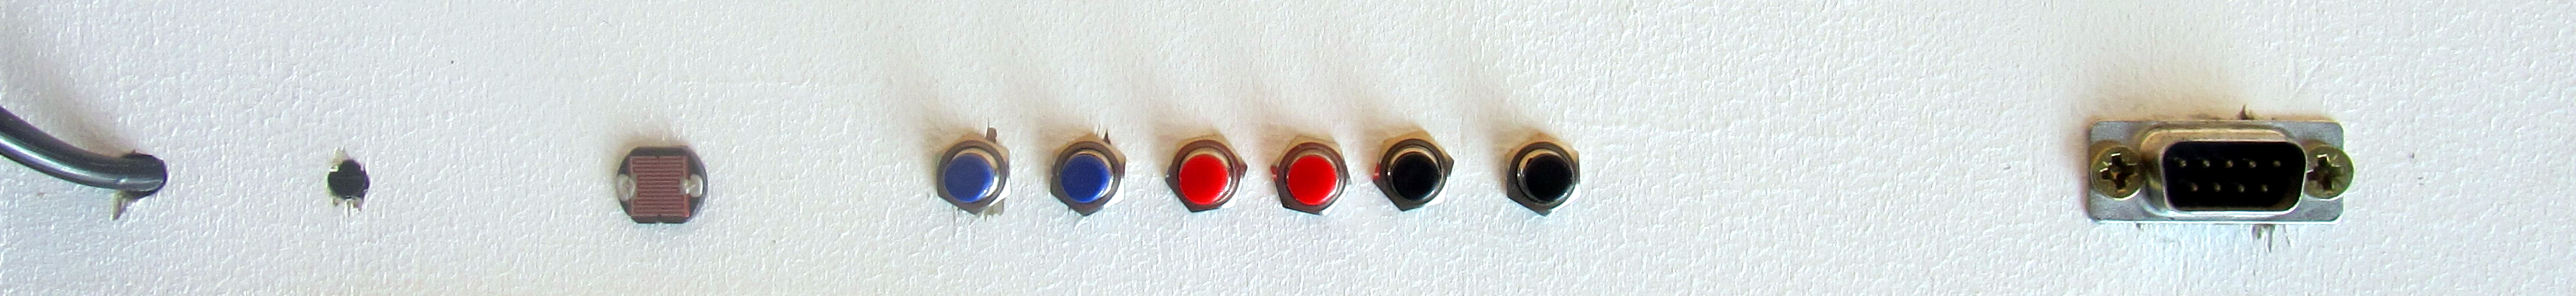
\includegraphics[width=\linewidth]{images/anschluesse.png}}
\captionof{figure}{Taster, Sensoren und ISP-Schnittstelle der Digitaluhr}\label{fig_anschluesse}
\vspace{.5em}
%TODO Fotos von dem ganzen Kram

Als Schrauben kamen Metallschrauben mit M5 %TODO 
Gewinde zum Einsatz. Die Muttern wurden in einem Holzblock befestigt, der anschließend mit der Rückwand verleimt wurde.%TODO: Abbildung? 
Diese Lösung zeichnet sich im Gegensatz zu Holzschrauben durch minimalen Verschleis aus und kann oft geöffnet und wieder verschlossen werden ohne Auszufransen.

\subsubsection{Energieversorgung und Verbrauch}
%TODO: Tabelle mit Alle AN/ Alle Aus/ Halb an. (eventuell mit neuen und alten Widerständen 
Als Netzteil wurde ein CE geprüftes 5V/2A Netzteil gewählt. Das kompakte verwendete Schaltnetzteil ist ausreichend dimensioniert um den, mit einem Labornetzteil, ermittelten maximalen Bedarf von ca. 1.8A%TODO
(alle LEDs an bei maximaler Helligkeit) bereitzustellen.
 
Als Stromkabel kommt ein zweipoliges Kabel mit Schalter zum Einsatz. Dieses wurde im Inneren des Gehäuses mit Schmelzklebestoff verklebt und in eine Lüsterklemme geführt, so dass bei eventuell auftretenden Zugkräften auf keinen Fall Kräfte auf das Netzteil wirken.

Mittels des Temperatursensors wurde außerdem in einem Testlauf sichergestellt, dass die Temperatur im Inneren der Uhr 50\degree C (bei einer Raumtemperatur von 22\degree C) nicht überschreitet.
%eof
	\section{Betrachtung des Gesamtsystems}
% Gehäuse
% Stromverbrauch
\subsection{Software-Architektur}
Die Software lässt sich in zwei Einheiten unterteilen:
\begin{itemize}
  \item zeitkritische Operationen
  \item nicht-zeitkritische Operationen
\end{itemize}
Zur Realisierung der zeitkritischen Operationen, wie dem Ticken der Uhr, dem Empfangen der Zeit sowie dem Ansteuern der LEDs wurden die Timer des AVR Microcontrollers benutzt. Der verwendetete Microcontroller ATmega32 besitzt drei Timer, einen 16-Bit- und zwei 8-Bit-Timer.

Die Timer senden in definierten Abständen Interrupts, die zur sofortigen Unterbrechung des Hauptprogrammes führen und den angegebenen Interrupt-Handler ausführen. Dazu wird der momentane Programmkontext auf den Stack gesichert, der Kontext für die Interrupt-Routine geladen, selbige ausgeführt und abschließend der Programmkontext wiederhergestellt, sodass die Ausführung des Programmes an der selben Stelle fortgeführt wird, wo es unterbrochen wurde. Unterbrechbar sind alle nicht-zeitkritischen Funktionen, die in einer Endlosschleife in der \texttt{main}-Methode des Programmes ausgeführt werden.

In den folgenden Unterkapiteln wird beschrieben, welche Funktion durch welchen Timer bzw. durch die Hauptschleife ausgeführt wird.
%
\subsubsection{Ansteuern der LEDs - Timer0}
Zum Ansteuern der LEDs wurde der 8-Bit Timer0 im \glqq Interrupt by Overflow\grqq -Modus verwendet. Dies bedeutet, dass er bei jedem Überlauf, also von $2^8-1$ auf $0$, einen Interrupt erzeugt. In dem Setup wurde ein 14,7456 MHz Quarz sowie ein Prescaler von 8 verwendet. Dies sorgt dafür, dass nur in jedem 8. Taktschritt der Zähler des Timers inkrementiert wird. Daraus resultiert eine Interruptrate von $\frac{Clock}{Prescaler * Steps} = \frac{14745600 Hz}{8 * 2^8} = 7200 Hz$. Dies bedeutet, dass die Funktion \texttt{static inline void drawWithBrightness(void)} 7200 mal in der Sekunde aufgerufen wird. Diese Funktion steuert bei jedem Aufruf eine Reihe von LEDs an und inkrementiert den Reihenzähler anschließend. Es entsteht also bei 7 Aufrufen der Funktion ein gesamtes Bild und damit ist die Bildfrequenz $\frac{7200 Hz}{7} \approx 1028,57 Hz$. Dies wirkt zunächst viel, wird aber durch die Pulsweitenmodulation (siehe \ref{sec_pulsweitenmodulation}) noch deutlich herabgesetzt.

\subsubsection{Ticken der Uhrzeit - Timer1}
Für die zeitlich kritischste Funktion, dem exakten Ticken der Uhrzeit wurde der 16-Bit Timer1 im \glqq CTC\grqq -Modus verwendet. CTC steht für Clear Timer on Compare Match und ist ein Modus, bei dem ein Höchstwert spezifiert werden kann, bei dem der Timer einen Interrupt auslöst und sofort wieder bei 0 zu zählen beginnt. Damit kann ein taktgenauer Timer realisiert werden, wodurch kaum Abweichungen in der Uhrzeit entstehen.

Es wurde sich dafür entschieden, als kleinste Zeiteinheit Dezisekunden zu verwenden. Zur Anzeige der Uhrzeit ist dies allemal ausreichend, aber so kann dieser Timer zusätzlich dazu verwendet werden, die Tasterzustände abzufragen und wäre für eine etwaige Anwendung, wo Dezisekunden benötigt werden (bspw. Stoppuhr) vorbereitet.

Um den Timer also 10 mal pro Sekunden einen Interrupt erzeugen zu lassen, muss der Vergleichswert folgendermaßen gesetzt werden: $CMP = \frac{Takt}{\frac{INT}{s}} = \frac{14745600 Hz}{10 \frac{1}{s}} = 1474560$. Dieser Wert kann von einem 16-Bit Timer nicht erreicht werden, da $2^16 < 1474560$. Deshalb muss auch hier ein Prescaler verwendet werden. Bei einem Prescaler von 1024 ergibt sich ein Wert von $\frac{1474560}{1024} = 1440$, welcher ideal ist, weil er einerseits innerhalb der 16-Bit Grenzen liegt und andererseits eine Ganzzahl ist, sodass genau bei jedem Interrupt eine Zehntelsekunde verstrichen ist.

Innerhalb der Timer1 Interruptroutine werden folgende Operationen ausgeführt:
\begin{enumerate}
  \item Die Uhrzeitvariablen (decisec, sec, min, hour) erhöhen
  \item Flag zum Messen der Helligkeit setzen
  \item Die Zeit neu in das Array zum Zeichnen schreiben
  \item Die Zustände der Taster abfragen
\end{enumerate}

\subsubsection{Empfangen der Uhrzeit - Timer2}
Der dritte Timer wird primär zum Empfangen der Uhrzeit verwendet, wird aber zusätzlich auch zur Tongenerierung für den Lautsprecher benutzt, wenn ein Alarm aktiv ist.

Auch dieser Timer wird im CTC-Modus verwendet, der Vergleichswert aber je nach Anwendung geändert. Beim Empfangen der Uhrzeit ist die Auflösung 10 ms und damit der $Vergleichswert = \frac{Takt}{Prescaler * \frac{INT}{s}} = \frac{14745600 Hz}{1024 * 100 \frac{1}{s}} = 144$. Innerhalb der Interruptroutine werden nun statusabhängige Funktionen zum Empfangen der Uhrzeit aufgerufen. Eine genauere Betrachtung dieser Funktionen ist in Kapitel \ref{sec_dcf77modul} zu finden.

Bei der Alarmfunktion wird der Wert abhängig der gewünschten Tonhöhe gesetzt.

\subsubsection{Nicht zeitkritische Funktionen in der main-Methode}
Alle Funktionen, bei denen die strikte zeitliche Einhaltung nicht wichtig ist, sind in der Hauptschleife des Programmes, einer \texttt{while(1)}-Schleife in der \texttt{main}-Methode zu finden.

Dort werden das Messen der Temperatur sowie der Helligkeit vorgenommen. Außerdem werden dort Events behandelt, die beim Drücken der Taster auftreten sollen, wie das manuelle Umstellen der Zeit oder der Helligkeit und zu guter Letzt die Verifizierung und Konvertierung der in Interruptroutine von Timer2 empfangenen Uhrzeit. Zusammenfassend also alles Funktionen, die für den Betrieb der Digitaluhr wichtig sind, bei denen es aber nicht darauf ankommt, wann genau sie aufgerufen werden, sondern nur, dass sie aufgerufen werden. 
%
%
%
%eof
	\section{Résumé}
\subsection{Evaluation}
In diesem Teil der Arbeit soll kritisch betrachtet werden in wie Weit die im
Teil Anforderungen gesetzten Ziele ereicht wurden.
\subsubsection{Modularität}
Die Uhr wurde Schritt für Schritt aufgebaut und hinzugekommene Funktionen
jeweils über Steckverbindungen mit der Hauptplatine verbunden. Sämtliche Module können
einzel getauscht/ersetzt oder weiterentwickelt werden. Besonders geschickt war
dies beim Austausch des DCF-Moduls, es konnte mit minimalen Änderungen von einem
Modul von Pollin zu dem höherwertigen Konrad Modul gewechselt werden. 
\subsubsection{Zeitempfang und Anzeige der Zeit}
Die grundlegendste Funktion der Uhr funktioniert wie geplant. Schwieriger als
gedacht hat sich dabei der Empfang der Uhrzeit herraus gestellt, da das
Empfangsmodul nicht immer korrekte Daten liefert. Durch fehlertolerante
Funktionen wird dieser Makel weitestgehend ausgeglichen und die Uhrzeit kann
korrekt Empfangen werden. Die 1 Sekunden Ticks der Uhr können, durch die Wahl
des Quarzes mit geeigneter Frequenz, mit hoher Genauigkeit eingehalten werden.
Auch die Anzeige der Uhrzeit wurde mit der LED Matrix wie gefordert umgestetzt,
als herrausragend erwies sich der geringe Stromverbrauch bei großer Helligkeit
der LEDs. Auch ermöglichten erst die LEDs eine Uhr in dieser Größe, da z.B.
sieben Segmentanzeigen nicht in dieser Größe verfügbar sind.

\subsubsection{Automatische Helligkeitsanpassung}
Das Zusammenspiel von Lichtsensor, Firmware und der LED Matrix mit ihren
Helligkeitsstufen funktioniert hervorragend. Verbessert werden könnte die
Funktion nur noch durch eine Durchschnittsfunktion über die Helligkeit und
unterschiedliche Schwellwerte für das Aufhellen und Abdunkeln der
Anzeige. Dadurch würde bei einer grenzwertigen Lichtstärke
nicht immer wieder zwischen den zwei entsprechenden Helligkeitsstufen hin und
her geschalten.
\subsubsection{Updatefähigkeit}
- externe ISP Schnittstelle über Stecker einer seriellen Schnittstelle 
- 

TODO: INCLUDE IMAGE OF BEAUTIFUL DIGITAL CLOCK HERE


\subsection{Weiterentwicklungsmöglichkeiten}
Die Grundfunktionalität der Uhr besteht nun und auch einige erweiterte
Funktionen, wie beispielsweise Temperatur- und Helligkeitsmessung sind
implementiert. Damit stellt das Projekt eigentlich einen abgeschlossenen Zustand
dar. Dennoch gibt es natürlich Erweiterungsmöglichkeiten. Es ist vorstellbar,
eine zukünftige Version mit Infrarotempfang auszustatten. So könnte man nicht
nur die Zeit eingeben, die Helligkeit kontrollieren oder einen Wecker vom Bett
aus bedienen, auch einfache Spiele wie das bekannte Pong wären denkbar. %Eine
% weiteres mögliches Zusatzfeature wäre eine externe Stromversorgung einzubauen.
% Man könnte beispielweise bei Auslösen des Weckers die externe Stromversorgung
% aktivieren, sodass ein Licht oder eine Musikanlage angesteuert wird.
Der ATmega
verfügt noch über 6 freie I/O - Pins, die für diese und weitere Erweiterungen
zur Verfügung stehen.

%Auch wenn diese Version der Uhr schon viele Funktionalität abdeckt, durch die selbstkonstruierte Bauweise sind viele Änderungen denkbar. Es wäre also durchaus der Anlass für eine zweite Version der Uhr gegeben.
%
\subsection{Fazit}
Diese Version der Uhr deckt viele Funktionalität ab. Wie aber im Kapitel Weiterentwicklungsmöglichkeiten erläutert wird, gibt es dennoch Raum für Erweiterungen, sodass eine zweite Version der Uhr durchaus denkbar wäre.
% Kosten

% Einleitung
% -Motivation
% -Umfang
% Anforderungen
% Technische Grundlagen
% - DCF77
% - LED Matrix
% - PWM
% Betrachtung der Komponenten
% - Mikrocontroller
% - DCF77 Empfangsmodul
% - LED Matrix
% - Helligkeitssensor
% - Temperatursensor
% - Infrarotempfänger
% Betrachtung des Gesamtsystems
% - Gehäuse
% Zusammenfassung
% -Evaluation
% -Weiterentwicklungsmoeglichkeiten
% -Fazit
% - Kosten


% NANANNANAN Matt\cite{cite1} Tobi\cite{cite2}
% 
% Uberblick gesamtsystem
% - Anfordungen an die Uhr
%  - elementar
%   - Zeitempfang
%   - Anzeigen der Zeit
%  - erweitert
%   - Datumsanzeige
%   - Wecker
%   - Helligkeitsanpassung
%   - geschaltet steckdose
%   - infrarotempfang
%   - temperatursensor
%   - Updatefaehigkeit
%   - Uhrzeit einstellen
%   
% -Betrachtung der einzelenen Elemente
%  - minimal
%  - erweitert
% -Display (LED Matrix)
%  - Prinzip
%  - Moeglichkeiten zur umsetzung
%  - vor und nachteile der Moeglichen
% - Zeitempfang
%  - DCF77 vs. GPS vs. England sender
%    GPS genauer aber teuerer, indoorempfang gut?
%  - DCF77 im Detail
%  - vergleich von verschieden empfangsmodulen
%  - vergleich von verschieden methoden zur auswertung
% - Mikrocontroller
%  - Warum mikrocontroller? und nicht fertiger baustein?
%  - ATmega vs. z.B. Cortex-m3 vs 
%  - Pro:
%   - einfache Programmierung
%   - guenstig
%   - einzeln verfuegbar
%   - DIP
%   - geringer stromverbrauch
%   - viele IO Pins
%   - viel verfuegbarer code
% 
%  
% - Zusatzmodule
%  - Temperatur
%   1 wire bus sensor um pins zu sparen und adc muss dann nicht umgeschaltet werden
%  - Helligkeit und dimmen
%   Lichtabhaeniger Widerstand an A/D Wandler und LED PWM
%  - Wecker
%   Lautsprecher + Weckzeit im EEPROM
%  - Steckdosenmodul
%   Relais mit verstaerkendem transistor/fet
%  - Infrarotmodul
%   Empfang und dekodierung von Infrarotsignalen von Fernbedienungen zur einstellung der Weckzeit
%  -
\newpage
\bibliography{Literatur/stud}
\bibliographystyle{geralpha}
\end{document}